\chapter{毫米波无线数据中心网络资源分配与优化研究}

\textbf{本章摘要:} 本章以无线数据中心网络为背景研究网状网络结构下的毫米波通信资源优化问题。研究在下一代数据中心网络中,利用毫米波高速无线传输代替传统的服务器间的有线连接,以提高数据中心网络的灵活性及可扩展性等性能。随着数据流量特性的变化,网络中不平衡流量逐渐增多,严重降低了DCN的通信性能。由于数据中心的机房环境相对稳定,服务器间位置也相对密集且固定,因此可以通过60GHz毫米波连接建立服务器间点对点的直接通信,以减少这些不平衡流量带来的通信性能下降。通过在每个柜顶(Top of Rack, ToR)布置毫米波阵列天线,建立了单层和三层两种数据中心无线网络拓扑结构,并提出了网络节点与邻居节点的生成方式。同时对建立的网络结构提出了天线资源分配优化算法,降低了整个系统中所有任务的最大传输时延。仿真结果验证了提出的毫米波无线数据中心网络结构与天线分配算法的有效性。

\textbf{关键词:}无线数据中心网络;毫米波通信;整数规划
%\keywords{无线数据中心网络;毫米波通信;整数规划}

\section{引言}
伴随着云计算(Cloud Computing)、大数据(Big Data)等技术的发展,用以储存、计算和传输海量数据的数据中心(Data Center) 的重要性越来越高,逐渐成为很多政府、公司的核心信息技术系统。数据中心通常有着固定的布局,在一个或几个房间内将服务器(Server)按照一定的规则布置在分层的机架(Rack)上,并将机架按照一定的模式固定在房间内。服务器之间依靠数据中心网络(Data Center Network, DCN)相互连接。
传统的数据中心主要采用有线的连接方式,通过一些固定的网络拓扑结构将服务器进行有效连接,其中比较著名的有Fat-tree\cite{al2008scalable}、BCube、DCell、Portland等结构。这些网络拓扑结构大多已应用在现有的网络中心并有着良好的性能表现,但都存在着一些类似的问题:
首先,有线连接需要大量的固定线缆及配套的温度管理设施,配线成本会占到设施成本的$8\%$左右\cite{popa2010cost},且线缆会占用大量数据中心的空气流动及冷却用空间,带来很高的设施成本。
其次,有线连接的线缆一般需要提前布置,大量的线缆接入时极易出错;同时网络拓扑结构也相应固定,将新的服务器连接到其余已有服务器时将会非常困难,即可扩展性较差。
此外,现有的数据中心网络流量存在着非常明显的流量不平衡现象\cite{benson2010network}:大约$80\%$的数据是那些传输延迟要求较高的小体量数据,而实际流量的大部分都集中在前$10\%$的那些吞吐量敏感的大体量数据上,也就是说流量矩阵实际上具有相当强的稀疏性,如图(\ref{fig:hs})所示。传统有线连接的数据中心网络拥有着相对固定且对称的网络架构,在面对这种极度不平衡的网络流量时,即使有冗余带宽的存在也仍然会出现通信热点(Hot Spot),显著降低数据中心网络性能。而如果针对这些潜在的通信热点建立超大带宽对等网络,则会带来巨大的资源消耗与浪费。

针对以上缺点,本章考虑使用无线连接的方式对传统数据中心网络进行升级,摆脱有线连接的缺点,以提高数据中心网络对非平衡流量的对应能力。
传统的无线解决方案如802.11a/b/g/n等系列由于传输速率的限制,难以满足服务器之间Gbps级的通信速率的要求。随着5G技术的研究发展,尤其是高速毫米波通信的应用,无线通信速率将会有显著提升,加之方向性信号传输带来的空间上干扰的降低,使用毫米波信号部分或者全部代替服务器/机架之间的有线连接将会是一个重要的发展趋势\cite{zhang2017free}。

使用毫米波信号进行服务器之间的无线通信拥有诸多好处:
\begin{enumerate}
\item 毫米波通信可以满足服务器之间的通信速率的要求:毫米波通信的通信速率一般为Gbps级以上,已有的利用60GHz频段进行通信的IEEE 802.11ad协议\cite{80211ad}(WiGig)已经可以达到7Gbps的通信速率。
\item 毫米波无线通信有着良好的可扩展性:增加、减少或是改变各个节点之间的拓扑结构都只需要改变波束的对准方向即可。
\item 由于毫米波信号快速衰减的特性使得信号传输的距离受到了限制,难以穿越墙体向外传播。这种性质在能满足一般数据中心的传输距离需要的同时,同时能利用数据中心周围的墙壁有效地避免数据信号被窃听,从物理上保证了数据的安全性。
\end{enumerate}

\begin{figure}[htbp]
\centering
\includegraphics[width=0.7\textwidth]{Pictures/Hotspot.pdf}
\caption{归一化后数据中心网络中的通信热点示意图\cite{kandula2009flyways}}
\label{fig:hs}
\end{figure}

因此本章设计将毫米波大规模天线阵列布置在服务器机架顶端,以建立毫米波无线数据中心网络,可以在一定范围内进行服务器架顶间的直接通信。如何设计毫米波无线数据中心网络结构,并对其中的资源进行合理分配与优化就成为热点研究问题之一。具体而言本章主要的贡献有以下几点:
\begin{enumerate}
\item 进行有线无线混合数据中心网络设计,在传统有线网络中心架构的基础上,通过在服务器机架顶配置毫米波无线天线以建立点对点通信的无线网络系统,解决数据中心网络中的通信热点问题。

\item 为了适应毫米波无线网络的传输特性,将数据中心网络的服务器放置方法进行改进,并在此基础上建立了单层及三层的无线网络拓扑结构,给出了不同情况下不同拓扑结构的节点与边的生成方式。

\item 在以上拓扑结构的基础上建立了天线资源优化问题,并通过同时优化分配接受和发射双方有限的天线资源,有效降低了系统的通信时延。
\end{enumerate}

本章其余部分组织如下:第4.2节介绍了数据中心网络领域的研究现状;第4.3节设计了系统模型,包括单层网络与三层网络两种拓扑结构;第4.4节提出了资源优化问题模型;第4.5节提出了收发双方天线资源优化分配方案;第4.6节利用仿真结果验证了所提出结构与算法的性能;最后,第4.7节总结本章。

\section{研究现状}

随着大数据,人工智能等科技应用的发展,数据中心网络流量由南北向流量为主转变为东西向流量为主,传统的三层有线数据中心网络逐渐暴露出设计上的缺点。主要表现在
\begin{enumerate}
	\item \textbf{流量受限}~为了降低传统数据中心网络的成本,通常采用带宽超额的方式,即通过使用不对等的上下行带宽以更有效的利用核心交换机的性能。然而当对应的工作量高峰时,核心交换机则会变成通信的瓶颈,造成数据拥堵。
	\item \textbf{低利用率}~由于预先铺设的通信设备带宽和端口数量均已固定,某些服务器节点处于空闲状态时,传输带宽难以被其他服务器利用,对应的线缆和服务器会带来巨大的浪费。
	\item \textbf{低扩展性}~在面对未来需要增加的服务器设备时,容易发生服务器端口不足的情况。此时传统的数据中心网络中一些核心节点就需要更换成拥有更多端口的设备,这会带来巨大的时间与金钱成本。
\end{enumerate}

光路交换机的引入大大提高了服务器间的传输带宽,但是由于数据中心出现的流量不平衡现象,通信热点带来的数据拥塞依然制约着数据中心网络性能的发展。为此近些年来,逐渐有学者提出混合有线/无线数据中心网络架构,将无线信号传输与传统有线数据中心网络相结合,在原有网络架构的基础上,通过加入点对点通信的无线网络通信甚至是全无线通信以提高数据中心网络的可扩展性,更好的应对数据流量不平衡现象。根据使用的无线通信介质的不同主要分为两大类\cite{hamza2016wireless},一类是通过自由空间光学传播(Free Space Optics, FSO)即无线光通信(Optical Wireless Communication, OWC)。另一类是通过毫米波信号无线射频信号的进行无线通信。其中FSO通信需要极为精确的校准以建立LoS通信链路,相对毫米波通信而言条件更为苛刻,因此本文将在毫米波通信的范围内进行研究。如图(\ref{fig:dcn1})展示了毫米波无线数据中心网络的几种链路传播方式。图A是利用角状天线进行数据通信。图B是利用天花板进行3D波束成形通信。图C是利用阵列天线波束成形进行通信。

%2014年Hamedazimi等人提出了Firefly\cite{hamedazimi2014firefly}架构,该架构认为完全自由的机架间网络可以在不需要任何核心交换机的前提下得到近乎最优的网络架构,可以提供双向对等的网络带宽。因此文章提出了全链接可重构的概念,将自由空间光学传播通信(FSO)应用到所有机架间链接上,机架内的服务器链接仍使用有线链接。利用自由空间光学传播的特性,在所有的机架顶配置FSO设备,并通过屋顶的镜面进行反射,以避免通信干扰。

2011年Daniel等人\cite{halperin2011augmenting}提出了利用60GHz毫米波无线通信提高传统有限数据中心网络的架构。通过使用方向性角状天线提高毫米波信号的传输效率,并将其传输到指定方向。在其前作\cite{kandula2009flyways}的基础上,相应的实验数据证明了60GHz毫米波信号在数据中心中传播的有效性。通过使用原型机对四种实际情况进行实验验证,证明了60GHz无线网络可以在数据中心中提供稳定的Gbps级别的通信带宽,将这种通信方式应用在某些热点通道上则可以显著地减少系统中的热点数量,减少了流量拥堵的情况,提高了数据中心网络的有效性。

\begin{figure}[htbp]
	\centering
	\includegraphics[width=0.85\textwidth]{Pictures/dcn1.pdf}
	\caption{无线数据中心网络示意图}
	\label{fig:dcn1}
\end{figure}

2012年Zhou等人提出了通过3-D波束成形算法,通过天花板反射的方式实现60GHz毫米波无线信号在数据中心网络的应用\cite{zhou2012mirror}。设计通过特制的金属面天花板进行一次反射,可以将数据中心内任意两个ToR连接,解决了60GHz毫米波通信通常面对的需要视距传播(LoS)的问题。

2013年Shin等人\cite{shin2013feasibility}提出了一种完全摒弃数据传输网络中的有线链接,采用全无线的通信架构。文章采用基于90-nm的CMOS技术\cite{pinel200960ghz}的60GHz方向性毫米波通信技术,可以支持小范围内的多个收发终端同时进行通信。同时放弃了传统的网络拓扑结构,建立了基于Cayley图\cite{prof1889theory}的全新架构。通过使用Y型交换机替代掉传统网卡设备,Cayley数据中心网络可以将圆柱形机架上的服务器间通信及机架间通信完全建立成网状结构,从而实现了全无线的数据中心网络。

2013年Cui等人提出在软件定义网络OpenFlow的框架下,应用60GHz毫米波无线通信与传统数据中心网络组成混合网络架构\cite{cui2013dynamic}。设计将无线通信应用于处于无线通信范围内的通信热点上,通过0-1信道连接矩阵构建无线传输图,利用基于范围的干扰模型计算无线传输之间的信干噪比SINR,并使用松弛方法解决了无线信道分配问题。

2014年Zhu等人提出了设备网络(Facilities Network)的概念,设备网络与数据平面正交,负责数据中心网络的控制平台以及设备的系统升级与安装。与传统的数据中心一个稳定的低延迟的无线数据中心架构\cite{zhu2014cutting}Angora。Angora提利用固定的方向性60GHz毫米波无线通信及波束成形技术提供稳定的路线解耦,并通过实验验证了60GHz毫米波通信的时延小于1毫秒,且可以保证相当长时间内的稳定传输,同时验证了在目的方向相差至少$12^{\circ}$时,干扰带来的吞吐量下降可以低至忽略不计。这也为60GHz毫米波通信波束成形技术在数据中心网络上的应用提供了实验基础。

Sree等人在2017年提出了一个服务器到服务器的无线数据中心网络\cite{umamaheswaran2017reducing},完全摒弃了数据中心的有线连接。在每个服务器上配备两个单独的角状天线,分别应用于水平向服务器通信与垂直向服务器通信。这种简化的通信方式能够保证始终存在视距传播的通信链路,但是在当需要通信的两个服务器不处于同一个水平或垂直平面上时,需要经过复杂的中继进行数据传输,带来了巨大的通信时延。

Zhang等人在2017年提出了另一种在数据中心网络中实现60GHz毫米波LOS视距传播的方式\cite{zhang2017free}。该方法借助于可升降(liftable)可旋转(rotatable)的曲柄支架以调节其上的毫米波天线,解决了视距路径阻隔的问题。同时设计提出了Graphite拓扑结构,将服务器架顶的天线按照一定模式分成多层,使得每层内部及多层之间都可以满足相当数量的服务器间视距传播,增加了节点的平均链接数量,并提高了数据中心网络系统的连接性,吞吐量以及传输质量。

Cui等人在2018年又提出了新的Diamond架构\cite{cui2018diamond},该架构摒弃了ToR的限制,通过在每一个服务器上配备一个无线终端,组成了高度可配置化的无线传输环。利用流线型的人型有线链接组成了低成本可扩展的3-D环状反射空间,使得无线信号可以在高精度的金属面进行多次反射。为支持大量并发的无线传输设计了精确的反射方式,金属面上大量覆盖了吸收材料,只有一些没有被吸收材料覆盖的小孔可以将信号高效的反射,极大降低了信号间的干扰。由于服务器和机架的位置是固定,因此金属板发射孔的位置可以事先设定,需要通信的两个终端间的天线发射和接收方向也可以提前设定,只需要查表即可得到相应的配置数据。

\section{系统模型}

毫米波信号由于其高频的特点在空间中衰减很快,同时很难穿过障碍物,且即使是镜面反射也会带来较强的衰减,因此通常使用视距传播的方式进行点对点毫米波通信。
在现有数据中心网络架构中,服务器间的有线连接能够满足正常流量的通信需求。但当出现大量不平衡流量时,大量数据需要通过某几个关键节点(交换机)进行转发,导致数据拥堵,出现通信热点的情况。因此本设计只考虑通信热点降低通信效率的情况,即正常的通信只需要通过已有的有线连接,毫米波无线点对点连接只应用于服务器/机架间点对点的数据传输。

本章研究在现有有线数据中心网络架构的基础上,应用60GHz毫米波无线信号进行服务器机架间的点对点通信,以应对DCN可能出现的通信热点问题。由于毫米波信号频率很高,在空间中衰减很快,因此通常采用方向性波束聚集信号能量。现有方向性波束的实现方法主要有两大类,一类是通过角状天线,如图(\ref{fig:horn}),另一类是通过自适应的智能阵列天线,如图(\ref{fig:macom})。应用于毫米波的角状天线口径一般在20-150mm左右,体积随着使用频率的提高逐渐减小,能够适应较宽的波段(12-325GHz)并很好地抑制旁瓣的生成,同时提供较为稳定的发射和接收增益。但是缺点在于旋转角度时需要通过机械装置的旋转,增加了波束旋转时延;同时通信增益限制在几个固定的增益值,难以实现实时动态的调整;而且由于机械结构的限制,难以实现一个服务器与多个其他服务器同时通信的要求;此外机械结构的稳定性与鲁棒性也难以保证。而自适应智能天线阵列只需要通过改变每个天线单元发射或者接收信号的相位,无需机械结构的转动即可实现波束转向(Beam Steering),可以带来毫米级的波束换向时延;同时在这种点对点通信的过程中,可以将所有可用天线单元资源进行虚拟分组,构成不同的子阵列与不同的服务器之间进行通信,一个服务器能够同时进行与不同服务器间的信号发射与接收,大大提高了数据中心网络架构的自由度;避免了角状天线只能与一个服务器同时通信的问题;同时发射和接收双方都拥有一定数量的天线组成的子阵列利用发射/接收波束成形技术进行通信,可以通过改变所使用天线阵列的天线数量动态的调整天线在某一方向上的发射/接收增益。因此本设计使用配置在各个服务器顶端的智能阵列天线进行毫米波方向性通信。

对于每一个服务器上的天线阵列使用相同的波束成形技术,当天线数量固定时,阵列天线的波束方向图(Beam Pattern)相对固定。如图(\ref{fig:60ghz})为由20个相同全向天线单元构成的均匀线性阵列使用60GHz频率进行通信,天线单元之间的距离为半个波长时的波束方向图。当使用天线单元数量增加时,所形成的波束主瓣会逐渐变细,增益也逐渐提高。因此在每个ToR总可用天线数量受限时,可以通过改变与不同服务器/机架通信所使用均匀线性子阵列的天线数量,动态调整数据中心网络中的带宽分配,减小通信热点带来拥堵,降低任务总通信时延。

\begin{figure}[htbp]
	\centering
	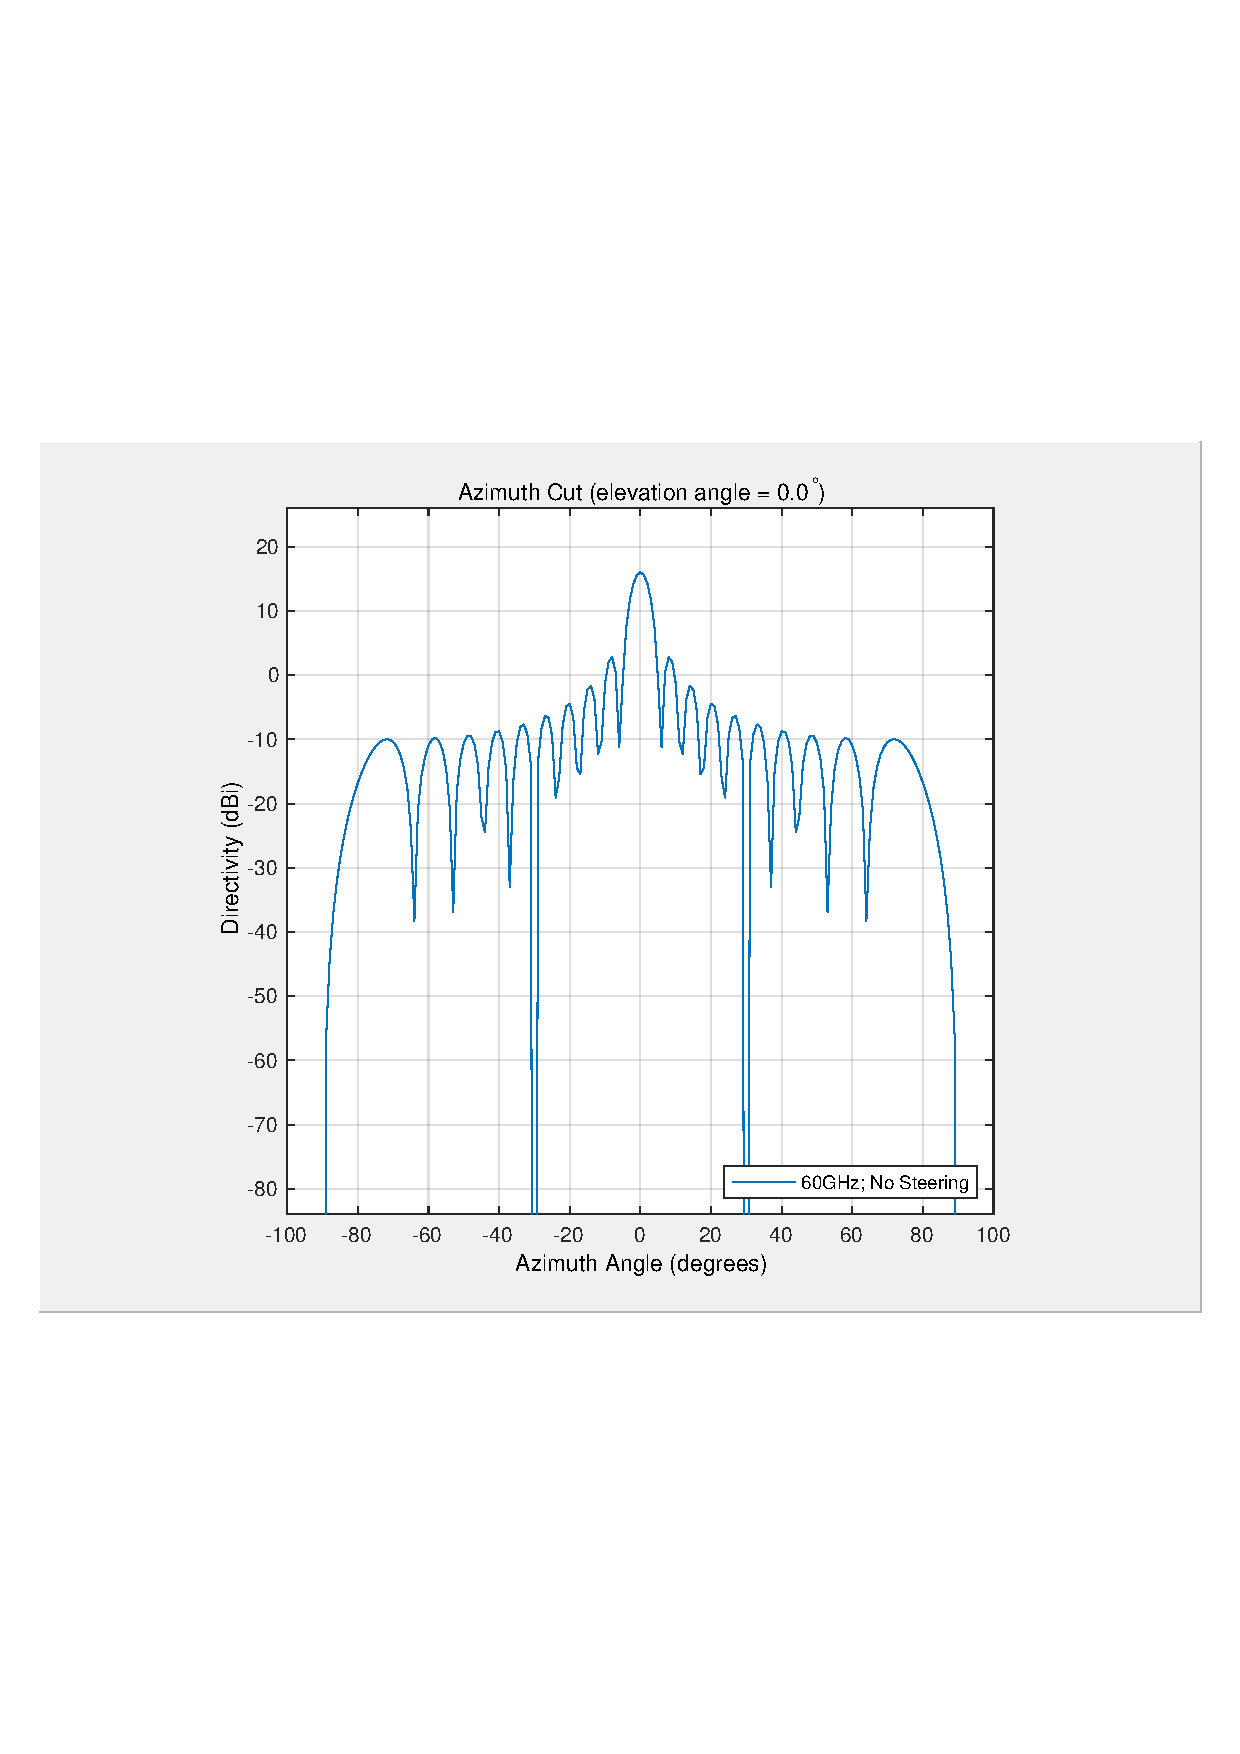
\includegraphics[width=0.7\textwidth]{Pictures/60GHz.pdf}
	\caption{包含20个天线单元的均匀线性阵列波束方向图}
	\label{fig:60ghz}
\end{figure}

\begin{figure}[htbp]
	\centering
	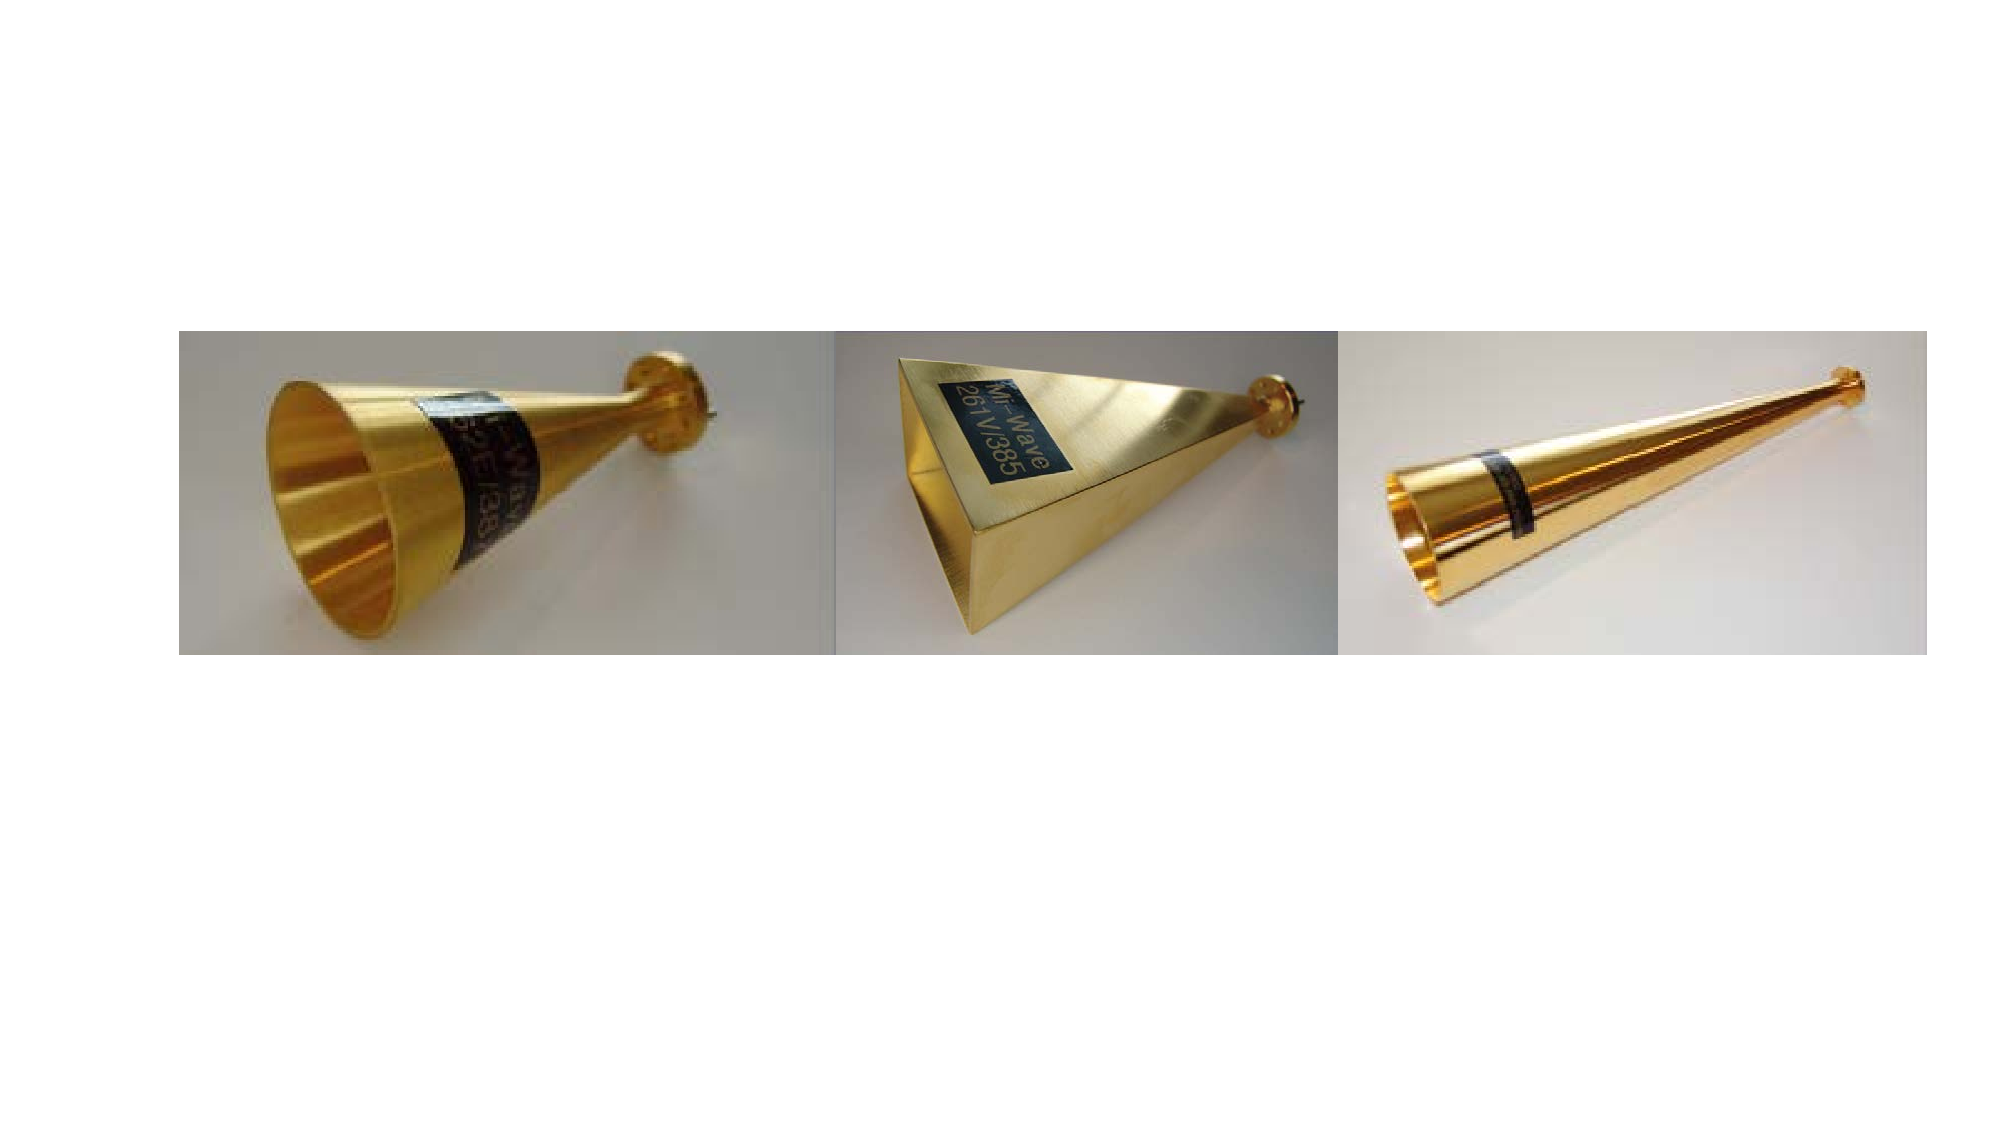
\includegraphics[width=0.7\textwidth]{Pictures/horn.pdf}
	\caption{几种用于毫米波通信的角状天线\cite{hornantenna}}
	\label{fig:horn}
\end{figure}

\begin{figure}[htbp]
	\centering
	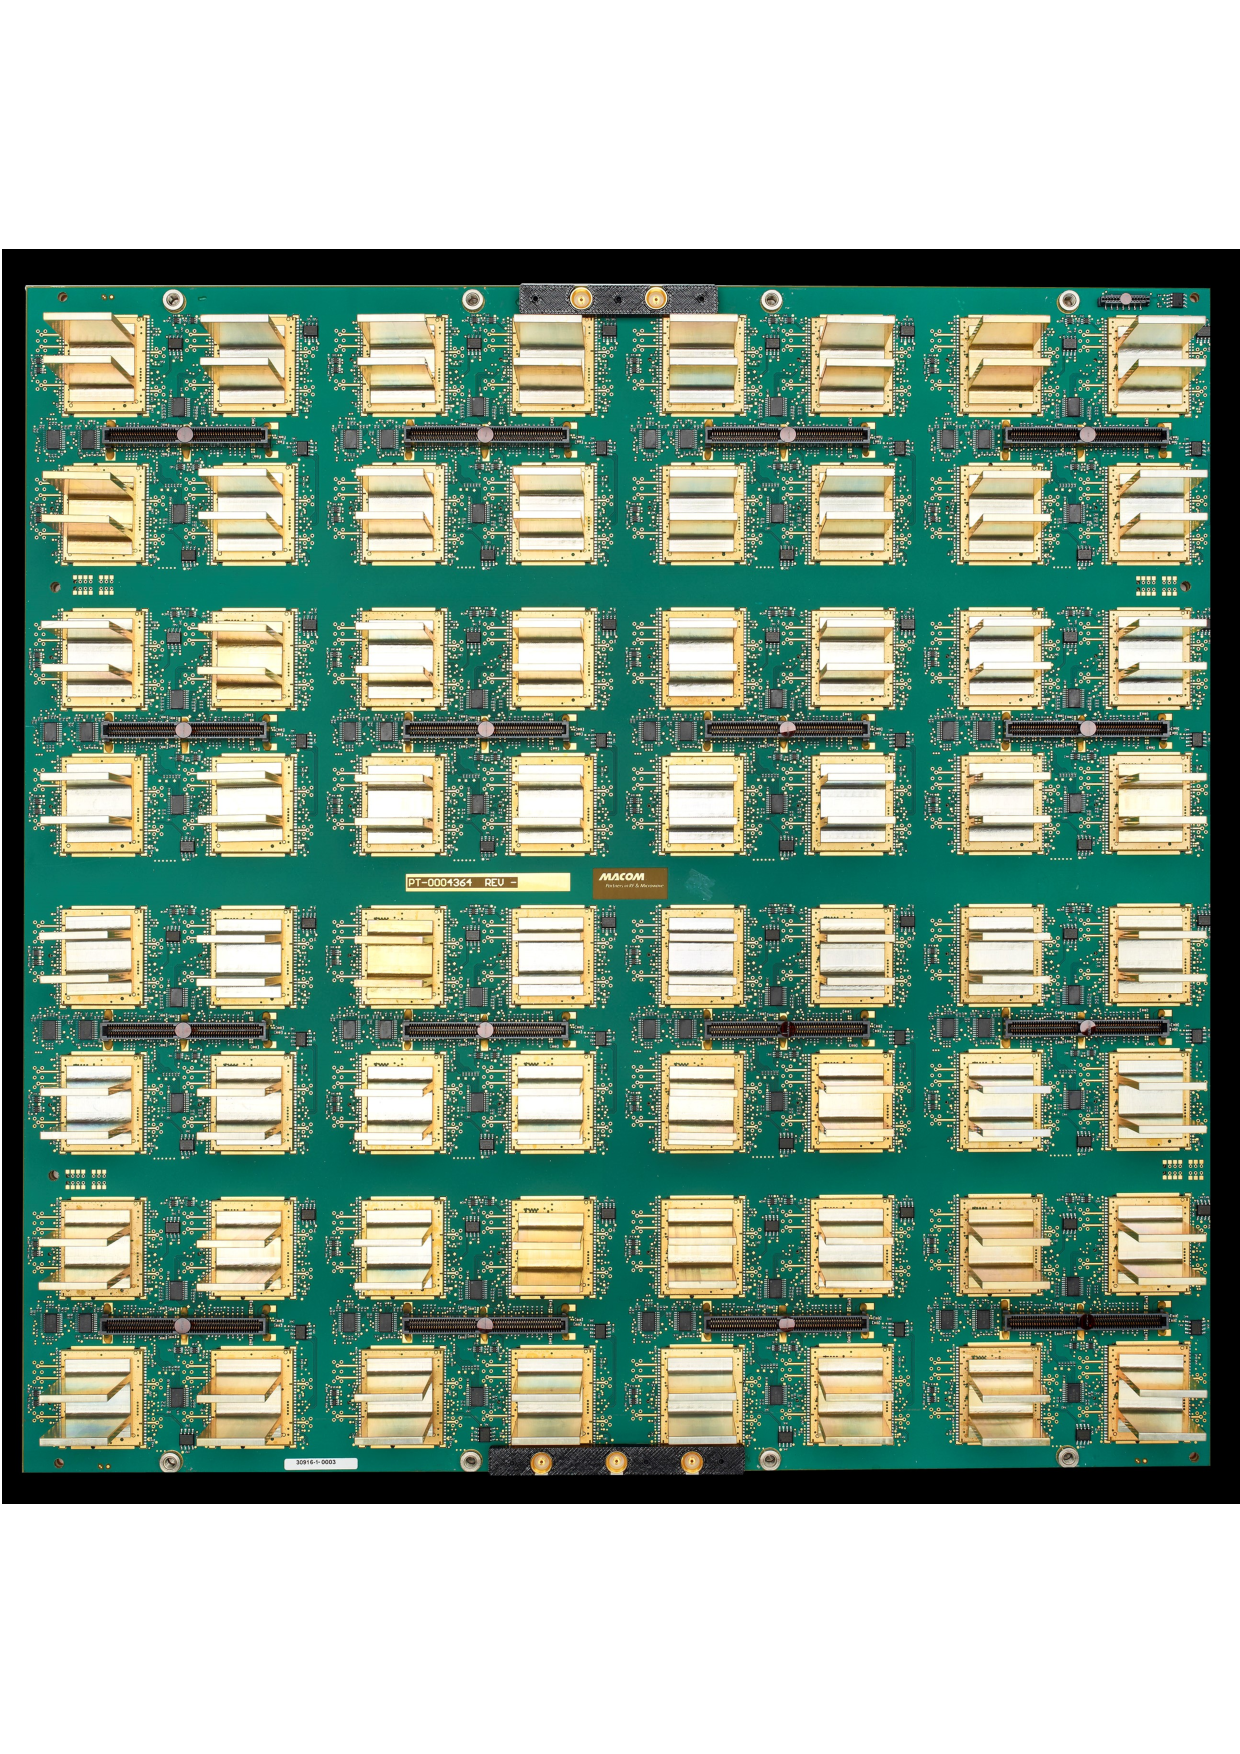
\includegraphics[width=0.6\textwidth]{Pictures/MACOM.pdf}
	\caption{包含64个天线单元的毫米波矩形天线阵列\cite{macom2017}}
	\label{fig:macom}
\end{figure}

本章考虑将传统服务器架顶结构与毫米波天线阵列相结合。传统服务器由于房屋容积,布线方便等原因通常采用成排的架构。这种排布方式会导致大量的服务器处于同一条直线上并互相阻挡视距传播路径。因此,传统的成排放置方式难以满足毫米波无线传输要求。由于只使用视距传播通信来保证通信的质量,就需要采用特殊的架构以得到尽量多的视距传播路径。
事实上,对于同一个天线阵列而言,发射/接收增益不仅收到所使用天线单元数量的影响,还会受到两个天线阵列间的相互角度即波束指向方向的影响。理论上波束转向的范围为$\theta \in (-90^{\circ},90^{\circ})$。而事实上,在波束方向接近与阵列平行(接近$-90^{\circ}$和$90^{\circ}$)时阵列增益会显著降低,这主要是由于天线的有效截面积的影响。即
\begin{equation}
	Gain = Gain_{idea} \times efficiency,
\end{equation}
其中
\begin{equation}
	efficiency \propto cos \theta.
\end{equation}
即波束角度越偏离均匀线性天线阵列的中垂线方向,实际的发射/接收增益就越小\cite{atesal2010x}。一般认为,当发射/接收波束与对应的均匀线形天线阵列的中垂线角度小于$60^{\circ}$时增益是有效的\cite{vardhan2014polycell}。
综合考虑毫米波视距传播与阵列间有效传输角度,采用六边形的服务器机架排布将会是合适的选择,如图(\ref{fig:hexagon})所示。将双面平面天线阵列以竖直方向安置在服务器机架顶端,且与服务器所在六边形的边平行。此时每个机架顶平面天线阵列能够与其所在两个相邻六边形上的所有架顶天线直接进行LoS通信。

\begin{figure}[htbp]
	\centering
	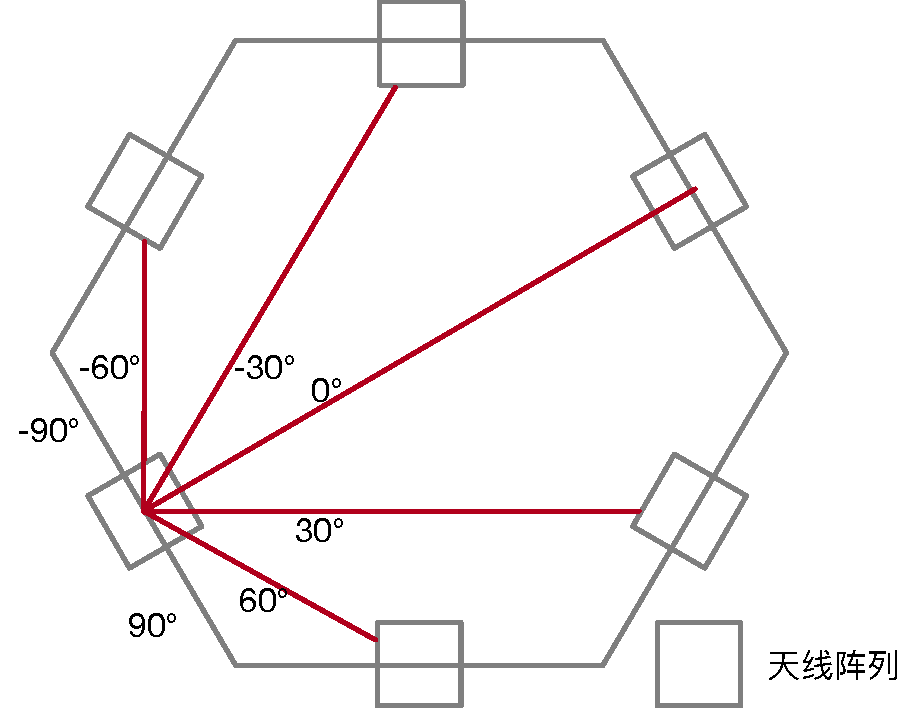
\includegraphics[width=0.7\textwidth]{Pictures/hexagon.pdf}
	\caption{服务器架正六边形网格放置时机架顶天线阵列的转向范围}
	\label{fig:hexagon}
\end{figure}

\section{无线网络拓扑结构}

为了建立完整的无线数据中心网络,需要分析无线链接的拓扑结构。本节介绍了两种网络的节点与边的生成方式,并分析了所组成网络拓扑的性能。

\subsection{单层网络拓扑结构生成}

对于六边形服务器放置架构,可以用图$G = (V,E)$来描述无线网络的拓扑架构。如图(\ref{fig:hexagon2})所示, 其中节点$V = \{ToR_1,ToR_2,...,ToR_N\}$为$N$个使用60GHz毫米波天线阵列,边
$E =\{e_{ij}:(i,j)\in S\subset[1,...,n]^2\}$为带权重$w_{ij}$的单跳有向链接,代表机架$i$发射到机架$j$的无线链路,其权重$w_{ij}$为机架$i$发射到机架$j$信号的实际带宽。ToR上的毫米波天线平面与所在蓝色线段平行,并垂直于地面放置。根据波束成形技术中的$60^{\circ}$有效角度,得到每个架顶天线只能与其所在的两个相邻的正六边形上的其余$10$个架顶天线相互通信,即图中红色架顶天线只能与周围的$10$个橙色架顶天线进行单跳信号双向传输。

\begin{figure}[htbp]
	\centering
	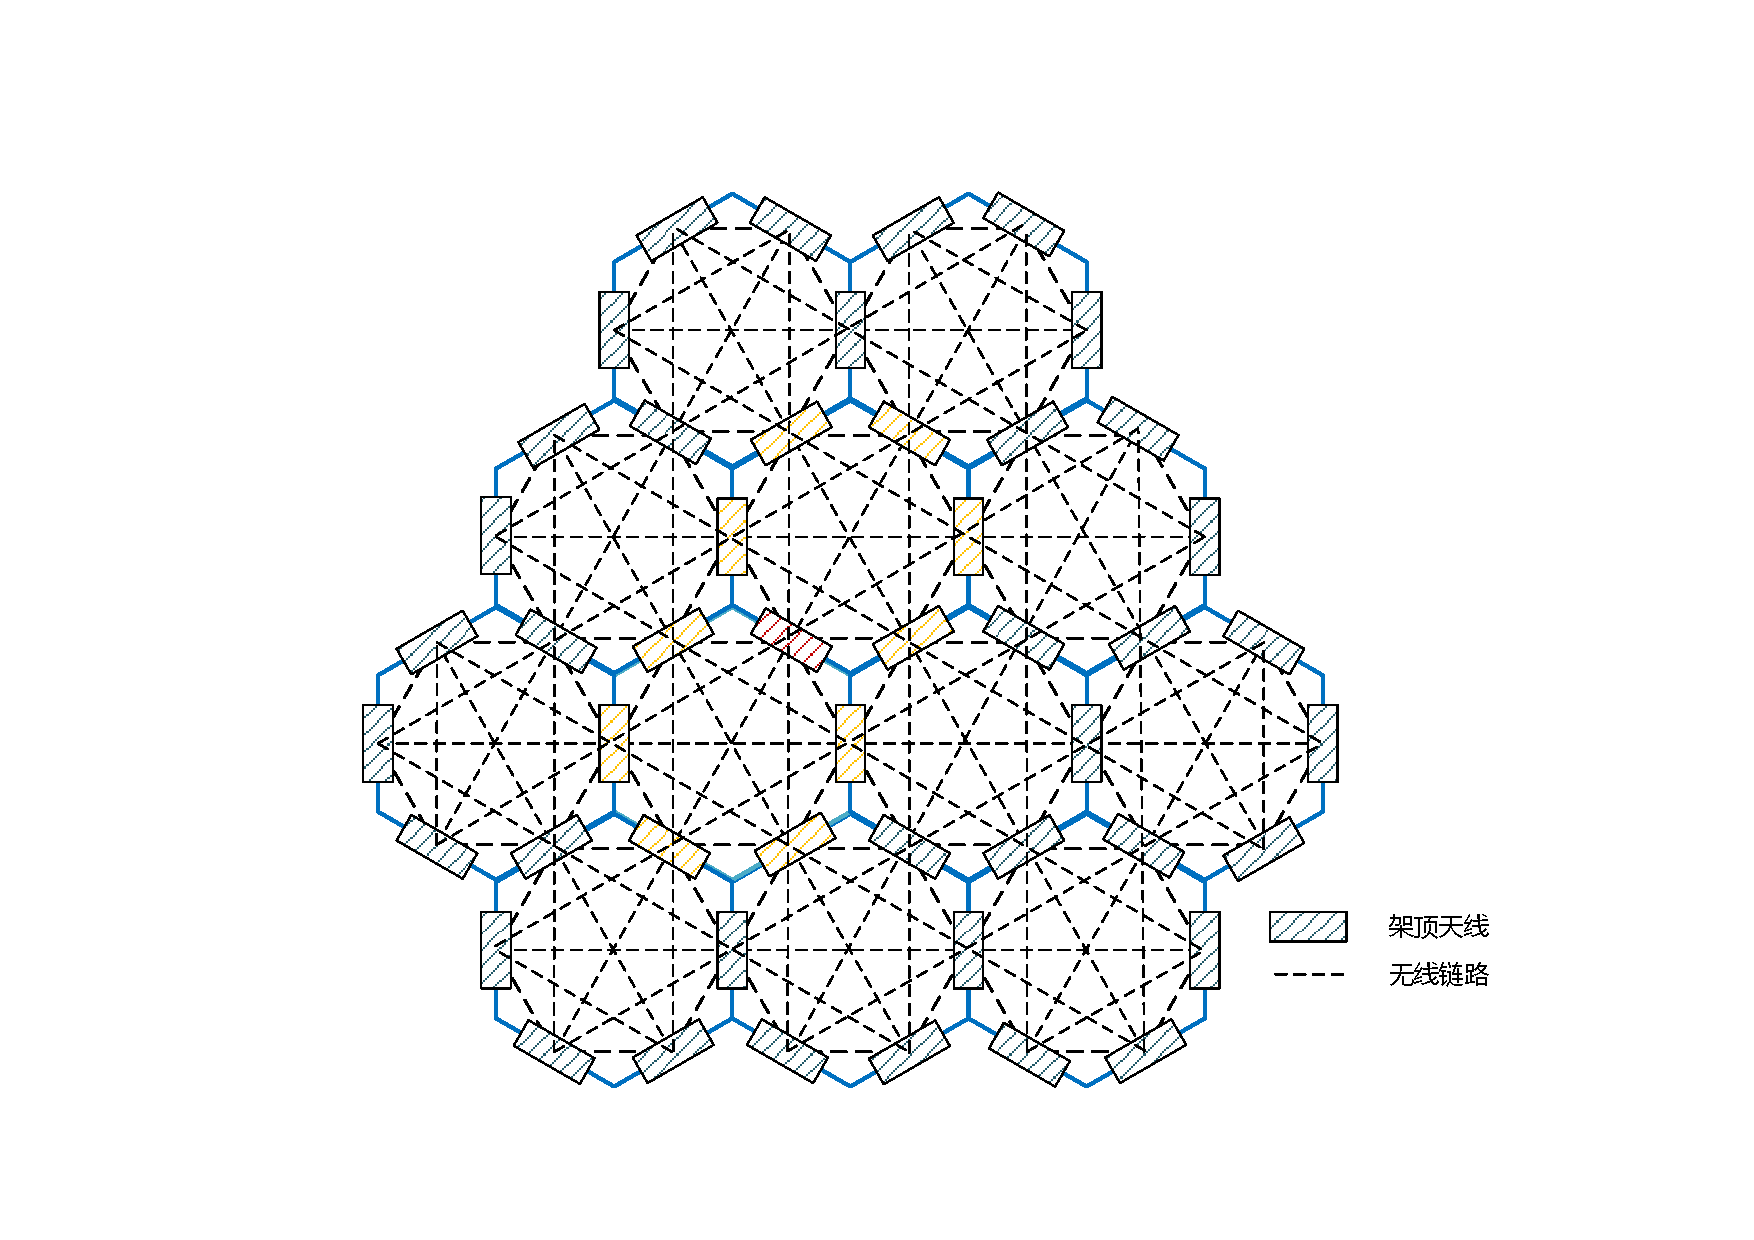
\includegraphics[width=0.7\textwidth]{Pictures/hexagon2.pdf}
	\caption{单层无线数据中心网络物理结构图}
	\label{fig:hexagon2}
\end{figure}

事实上天线之间的无线链接是带有权重$w_{ij}$的有向边,且该权重由发射和接收双方即边的两个端点共同决定并可以随时改变。为了分析网络的拓扑结构,可以先将权重忽略以简化分析。单层的无线数据中心网络中的节点可以通过基于Axial Coordinates的方式生成。具体如算法(\ref{alg:4.1})所示

\begin{algorithm}
	\SetAlgoLined
	\caption{单层无线数据中心网络拓扑结构节点生成算法} \label{alg:4.1}
	\textbf{初始化:}初始正六边形中心位置$(0,0)$,单位方向$\vec x_0$,$\vec y_0$分别从中心指向初始六边形两个相邻边的中点\;
	基于Axial Coordinates坐标生成六边形网格,其中所有六边形的中心点集合为$A = \{a_{x,y}\}$\;
	\ForEach{$x \in \mathbb{Z},y \in \mathbb{Z}$}
	{
		$C = \{ v_{x,y}|x = 2i+1 ~\&\&~ y = 2j, ~~ i,j \in \mathbb{Z} \}$\;
		$V = \{v_{x,y}\} = A-C$\;
	}
	\textbf{输出:}$C,V$
\end{algorithm}

在服务器所在机架的节点生成后,每个节点$c_{x,y}\in C$周围的六个节点$v_{x,y}$可以组成一个新的正六边形,且每个节点$v_{x,y}$都处于两个相邻新六边形公共边的中点。令任意两个机架间的最小距离为基础距离d$0$,天线的最大通信距离小于$3$倍的d$0$。为了得到每个节点的邻居节点,需要判断其所在的公共边的朝向。具体如算法(\ref{alg:4.2})所示。此时拓扑结构中的边为$E :={\{v,N(v)\} }$。

\begin{algorithm}
	\SetAlgoLined
	\caption{单层无线数据中心网络拓扑结构邻居节点寻找算法} \label{alg:4.2}
	\textbf{初始化:}初始正六边形中心位置$(0,0)$,单位方向$\vec x_0$,$\vec y_0$分别从中心指向初始六边形两个相邻边的中点,算法(\ref{alg:4.1})得到的集合$V=\{v_{x,y}\}$\;
	\ForEach{$x \in \mathbb{Z},y \in \mathbb{Z}$}
	{
		\uIf{$x$ is even $~\&\&~$ $y$ is odd}{
			$N(v_{x,y}) = \{v_{x,y-1},v_{x+1,y-2},v_{x+2,y-2},v_{x+2,y-1},v_{x+1,y},v_{x,y+1}$\,
			$v_{x-1,y+2},v_{x-2,y+2},v_{x-2,y+1},v_{x-1,y}\}$
		}
		\uElseIf{$x$ is even $~\&\&~$ $y$ is even}{
			$N(v_{x,y}) = \{v_{x+1,y-1},v_{x+2,y-1},v_{x+2,y},v_{x+1,y+1},v_{x,y+1},v_{x-1,y+1}$\,
			$v_{x-2,y+1},v_{x-2,y},v_{x-1,y-1},v_{x,y-1}\}$
		}
		\ElseIf{$x$ is odd $~\&\&~$ $y$ is odd}{
			$N(v_{x,y}) = \{v_{x+1,y},v_{x+1,y+1},v_{x,y+2},v_{x-1,y+2},v_{x-1,y+1},v_{x-1,y}$\,
			$v_{x-1,y-1},v_{x,y-2},v_{x+1,y-2},v_{x+1,y-1}\}$
		}
	}
	\textbf{输出:}$v_{x,y}$的邻居节点$N(v_{x,y})$。
\end{algorithm}

以上过程如图(\ref{fig:topology})所示,黄色圆点代表服务器机架位置,红色直线代表该点与其相邻节点的边。每个黄色圆点上的坐标可以惟一确定一个服务器机架的位置,如$(0,-1)$点惟一确定服务器$v_{0,-1}$。可以发现处于非边界上的节点的度为$10$。

\begin{figure}[htbp]
	\centering
	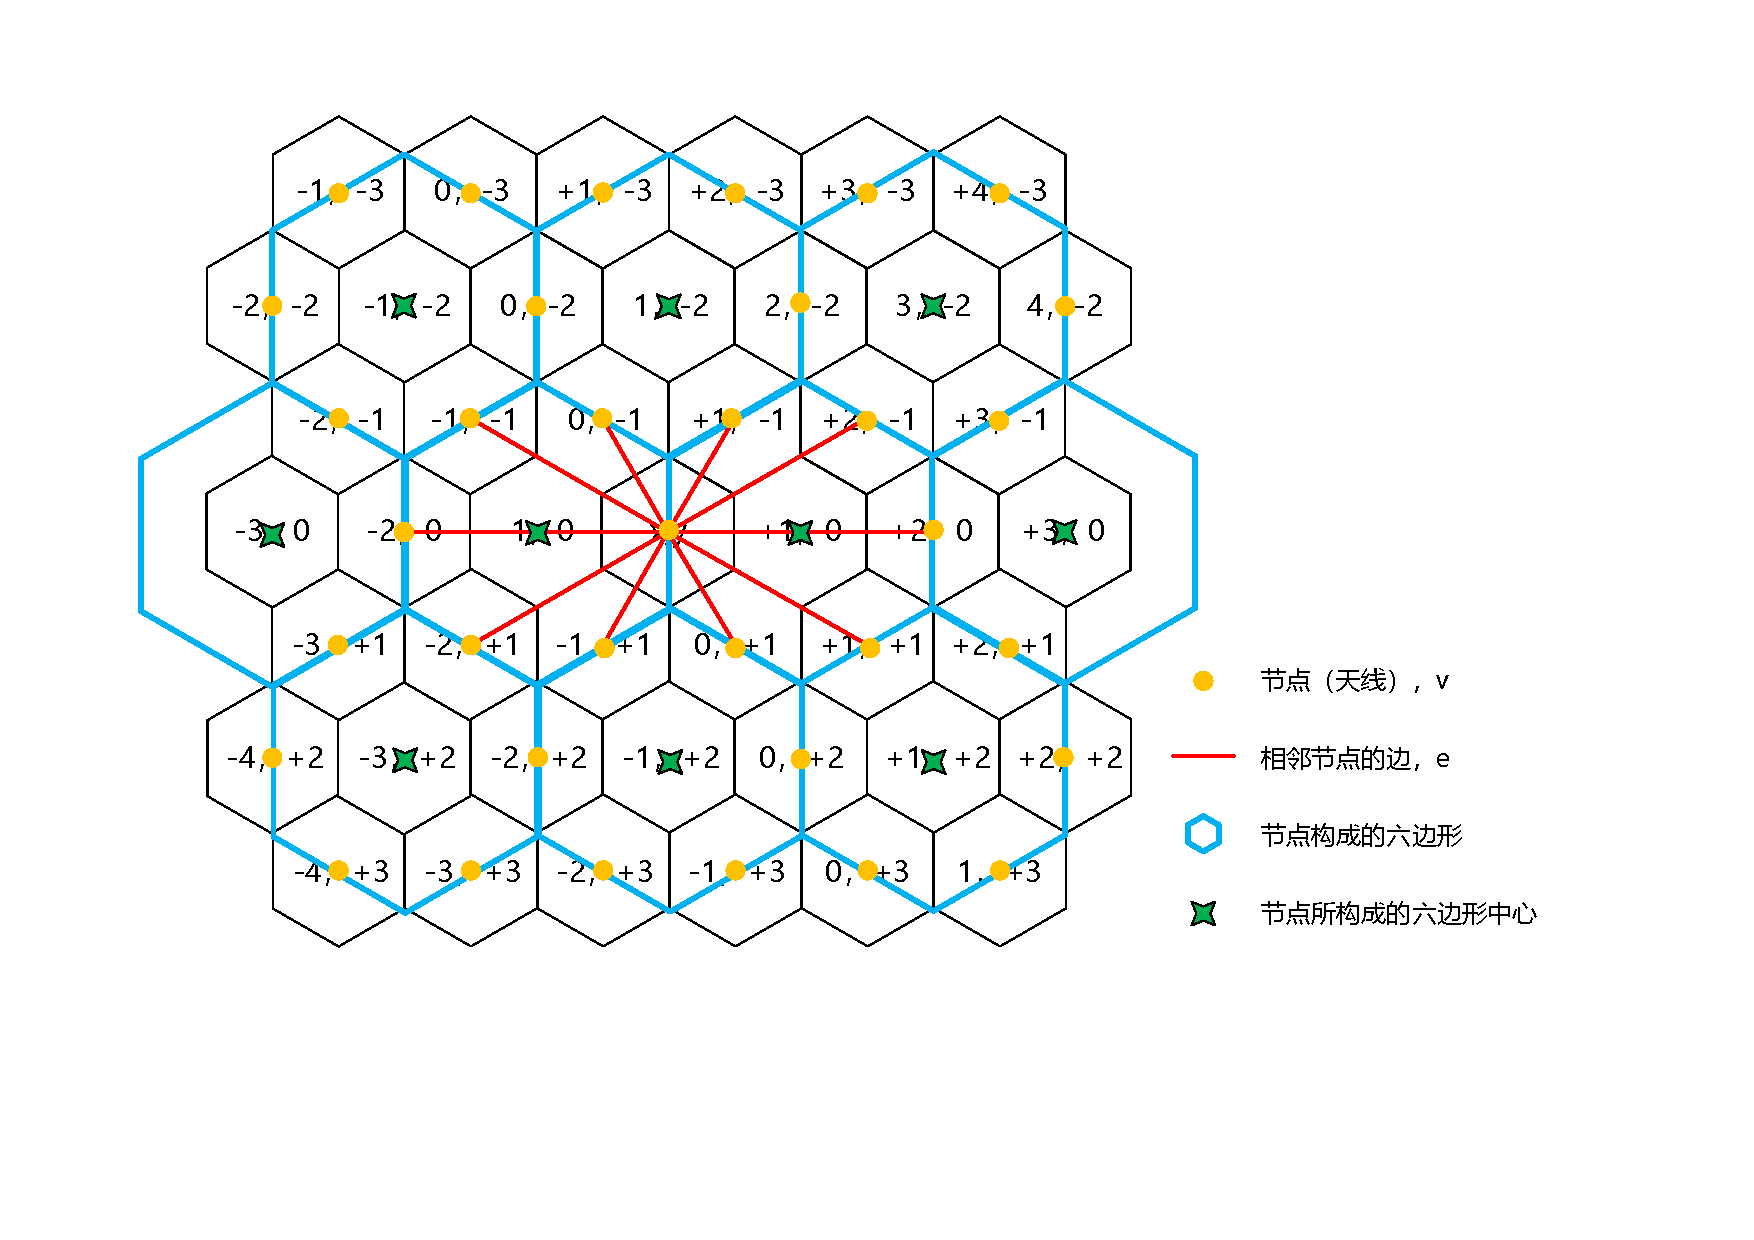
\includegraphics[width=0.8\textwidth]{Pictures/topology.pdf}
	\caption{节点、邻居节点和边形成示意图}
	\label{fig:topology}
\end{figure}

\subsection{三层网络拓扑结构生成}

当所有天线都处于同一个水平面时,在俯视图上处于同一条直线上的天线阵列将会互相阻挡。此时可以通过将机架顶天线置于不同高度的水平面以减少相互间的阻挡。考虑到六边形网格形状特点,将天线分成三层布置是一种合适的选择。如图(\ref{fig:3layer}),将全体节点按照一定规律分成三个平面布置,每层天线的相对高度分别为$h1,h2,h3$,每三个相互距离最近的节点处于不同的层。此时每层之间的临近节点可以直接相互通信,不同层之间的节点在距离较近时也可以不受阻碍的进行视距通信,如图(\ref{fig:hexagon3})所示。
依照算法(\ref{alg:4.3})可以生成三层节点$V_1,V_2,V_3$,其中同一层的节点处于同一个水平面内。

\begin{figure}[htbp]
	\centering
	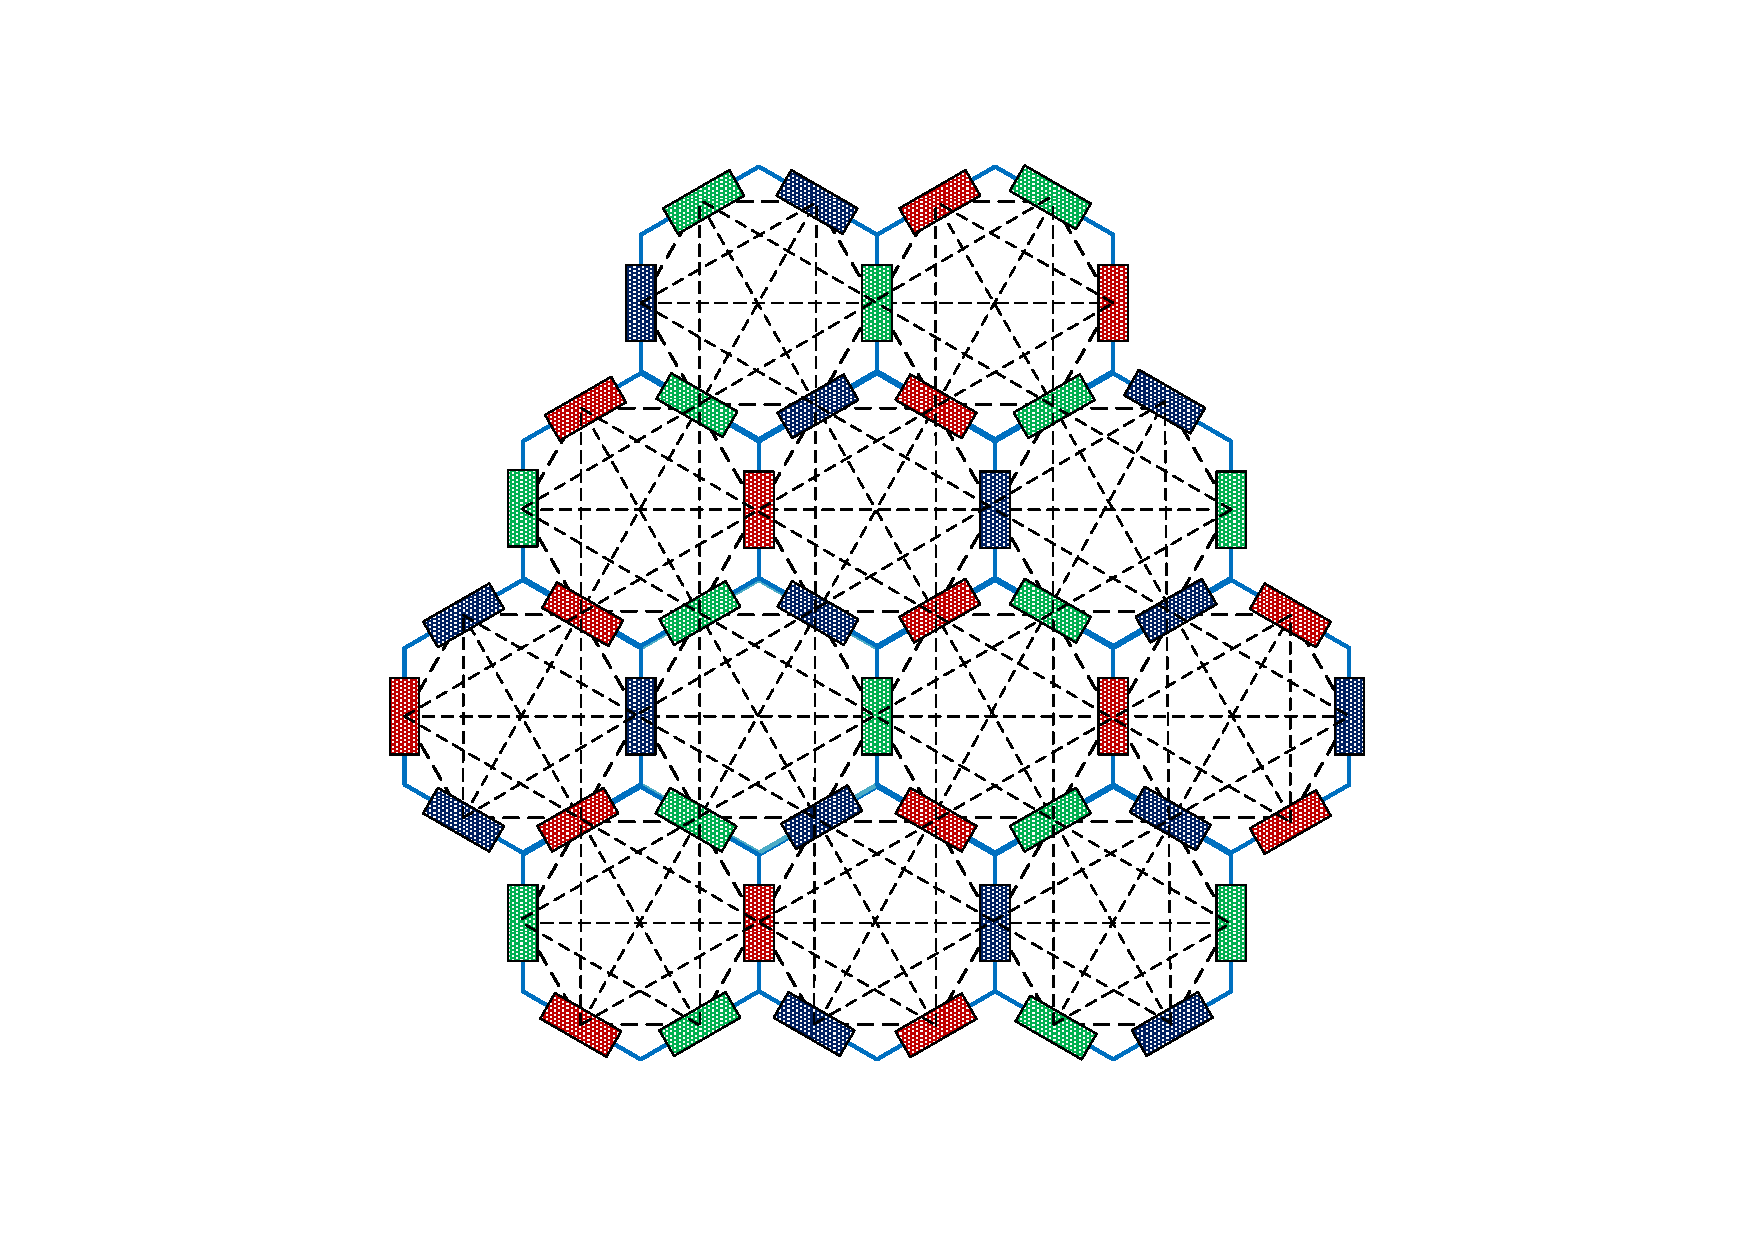
\includegraphics[width=0.7\textwidth]{Pictures/hexagon3.pdf}
	\caption{三层无线数据中心网络结构图}
	\label{fig:hexagon3}
\end{figure}

\begin{figure}[htbp]
	\centering
	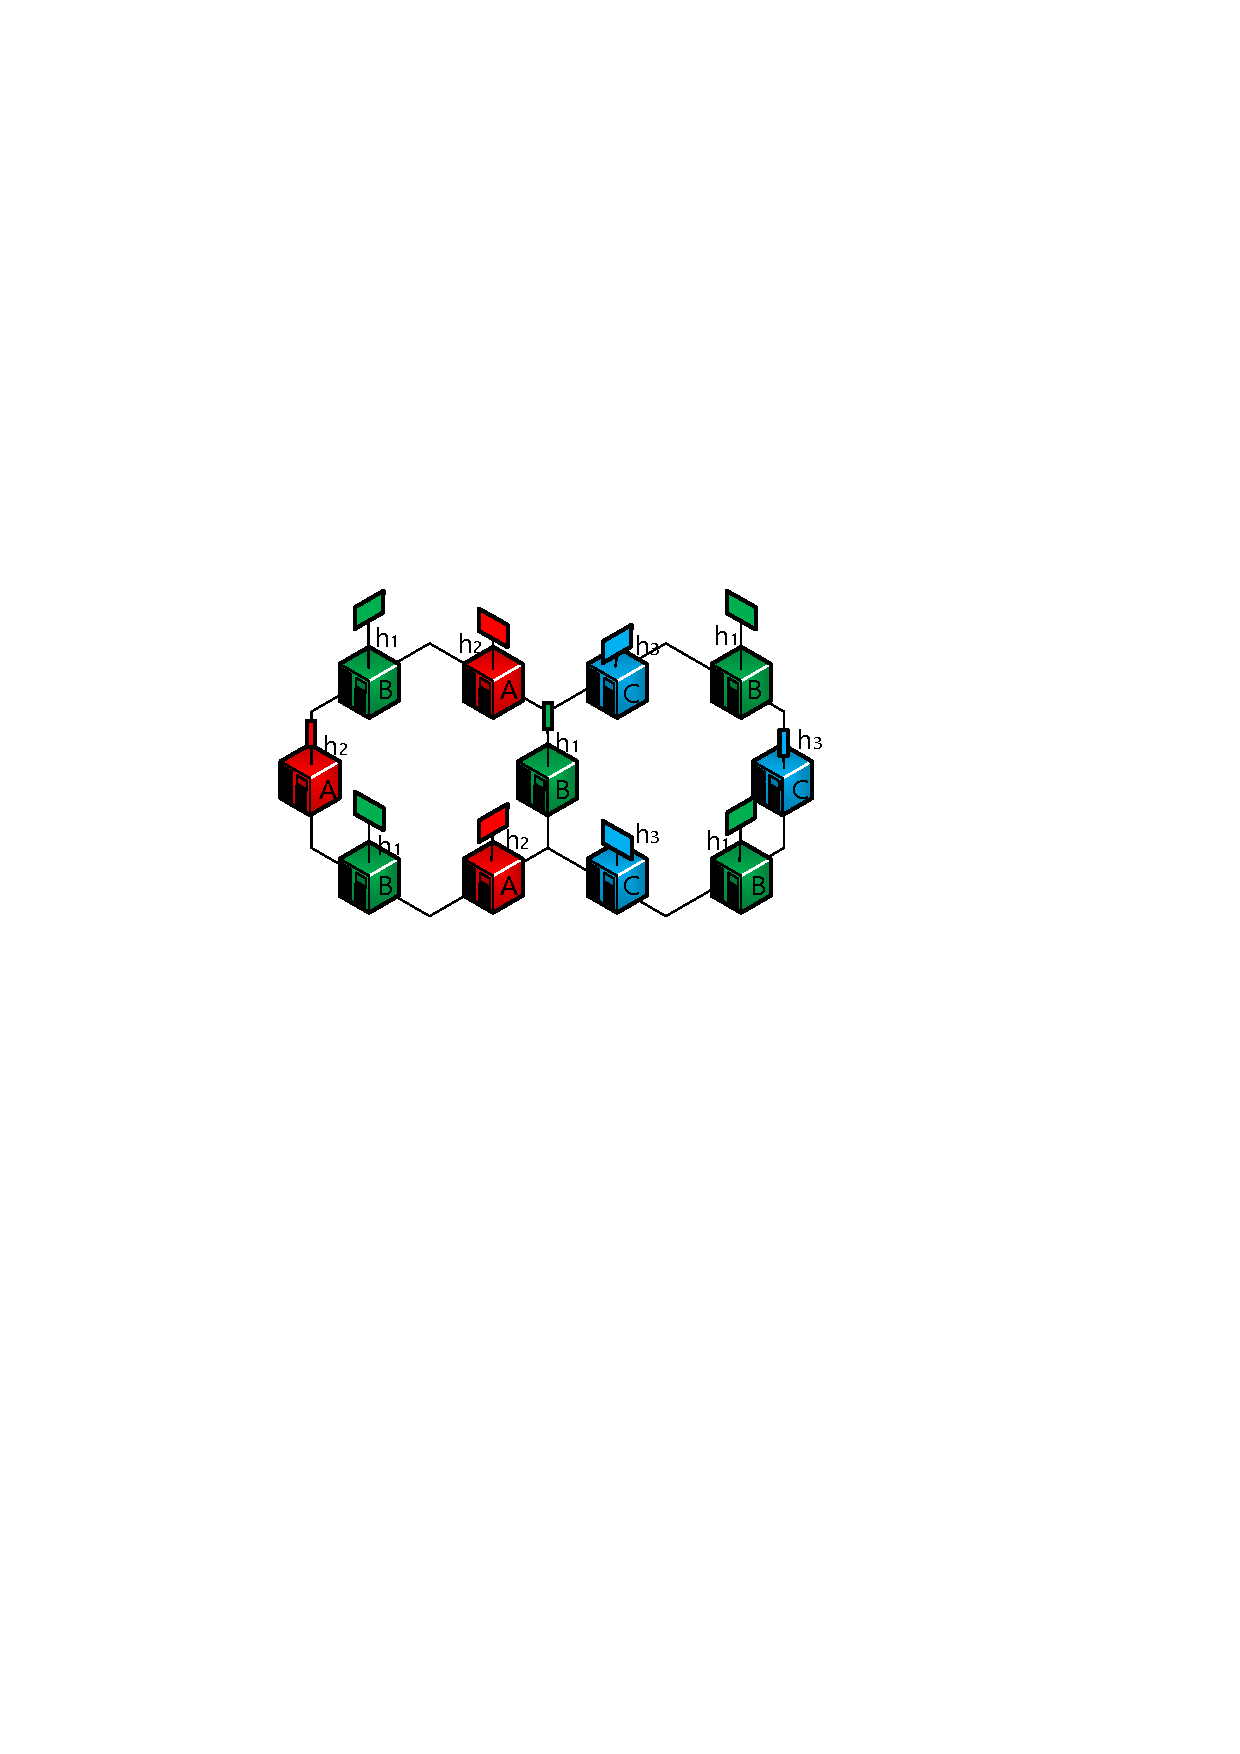
\includegraphics[width=0.7\textwidth]{Pictures/3layers.pdf}
	\caption{三层无线数据中心机架布置图}
	\label{fig:3layer}
\end{figure}

\begin{algorithm}
	\SetAlgoLined
	\caption{三层无线数据中心网络拓扑结构节点生成算法} \label{alg:4.3}
	\textbf{初始化:}初始正六边形中心位置$(0,0)$,单位方向$\vec x_0$,$\vec y_0$分别从中心指向初始六边形两个相邻边的中点,
	算法(\ref{alg:4.2})生成的节点集合$V,C$\;
	\ForEach{$x \in \mathbb{Z},y \in \mathbb{Z}$}
	{
	\uIf{$y$ is even}{
		$V1 = \{V|x = 6i + y,~ i \in \mathbb{Z}\}$\;
		$V2 = \{V|x = 6i + 2 + y,~ i \in \mathbb{Z} \}$\;
		$V3 = \{V|x = 6i + 4 + y,~ i \in \mathbb{Z} \}$\;
	}
	\ElseIf{$y$ is odd}{
		$V1 = \{V|x = 3i + y,~ i \in \mathbb{Z}\}$\;
		$V2 = \{V|x = 3i + 2 + y,~ i \in \mathbb{Z} \}$\;
		$V3 = \{V|x = 3i + 4 + y,~ i \in \mathbb{Z} \}$\;
	}
	}
	\textbf{输出:}$V1,V2,V3$
\end{algorithm}

与单层网络情况类似,在俯视图上每个节点$c_{x,y}\in C$周围的六个节点$v_{x,y}$可以组成一个新的正六边形,且每个节点$v_{x,y}$都处于两个相邻新六边形公共边的中点。由于每三个相互距离最近的节点处于不同的层,使得每个节点的视距传播范围中增加了单层网络结构中不能进行视距传播的若干节点。这些节点包括原来在同一条直线上而现在处于不同平面的节点,但是不包括那些虽然不被阻挡但是仍处于通信盲区($\theta \in (-90^{\circ},-60^{\circ})$ 或 $\theta \in (60^{\circ},90^{\circ})$)的节点。当然,邻居节点的数量同时收到最大通信距离的影响,当天线的最大通信距离小于$3$倍的d$0$时,可以依照算法(\ref{alg:4.4})的方法生成邻居节点。此时拓扑结构中的边为$E :={\{v,N(v)\} }$。

\begin{algorithm}
	\SetAlgoLined
	\caption{三层无线数据中心网络拓扑结构邻居节点寻找算法} \label{alg:4.4}
	\textbf{初始化:}初始正六边形中心位置$(0,0)$,单位方向$\vec x_0$,$\vec y_0$分别从中心指向初始六边形两个相邻边的中点,算法(\ref{alg:4.3})得到的集合$V1,V2,V3$\;
	\ForEach{$x \in \mathbb{Z},y \in \mathbb{Z}$}
	{
		\uIf{$x$ is even $~\&\&~$ $y$ is odd}{
			$N(v_{x,y}) = \{v_{x,y-1},v_{x+1,y-2},v_{x+2,y-2},v_{x+2,y-1},v_{x+1,y},v_{x,y+1},v_{x-1,y+2},v_{x-2,y+2}$\,
			$v_{x-2,y+1},v_{x-1,y},v_{x-2,y},v_{x+2,y},v_{x,y-2},v_{x,y+2}\}$
			%$v_{x-2,y+1},v_{x-1,y},v_{x-2,y}+v_{x-3,y},v_{x+2,y},v_{x+3,y},v_{x,y-2},v_{x,y-3},v_{x,y+2},v_{x,y+3}\}$
		}
		\uElseIf{$x$ is even $~\&\&~$ $y$ is even}{
			$N(v_{x,y}) = \{v_{x+1,y-1},v_{x+2,y-1},v_{x+2,y},v_{x+1,y+1},v_{x,y+1},v_{x-1,y+1},v_{x-2,y+1},v_{x-2,y}$\,
			$v_{x-1,y-1},v_{x,y-1},v_{x,y-2},v_{x,y+2},v_{x-2,y+2},v_{x+2,y-2}\}$
			%$v_{x-1,y-1},v_{x,y-1},v_{x,y-2},v_{x,y-3},v_{x,y+2},v_{x,y+3},v_{x-2,y+2},v_{x-3,y+3},v_{x+2,y-2},v_{x+3,y-3}\}$
		}
		\ElseIf{$x$ is odd $~\&\&~$ $y$ is odd}{
			$N(v_{x,y}) = \{v_{x+1,y},v_{x+1,y+1},v_{x,y+2},v_{x-1,y+2},v_{x-1,y+1},v_{x-1,y},v_{x-1,y-1},v_{x,y-2}$\,
			$v_{x+1,y-2},v_{x+1,y-1},v_{x-2,y},v_{x+2,y},v_{x-2,y+2},v_{x+2,y-2}\}$
			%$v_{x+1,y-2},v_{x+1,y-1},v_{x-2,y},v_{x+2,y},v_{x+3,y},v_{x-2,y+2},v_{x-3,y+3},v_{x+2,y-2},v_{x+3,y-3}\}$
		}
	}
	\textbf{输出:}$v_{x,y}$的邻居节点$N(v_{x,y})$
\end{algorithm}

显然这种拓扑结构会随着机架间的基础距离改变或是天线通信范围改变而发生变化。当两者比例变大时,节点的邻居节点数量会下降;当两者比例变小时,邻居节点数量将会上升。

\subsection{网络参数分析}

两个网络中边的权重都是可变的,对此只分析在无权重情况下的网络参数。
当通信距离小于等于$3$倍机架基础距离时,单层无线网络拓扑结构的平均度$K_1$为
\begin{equation}
	K_1= \frac{1}{|V|}\sum_{v\in V}deg(v) = 10,
\end{equation}
其中忽略了节点的边缘效应。在不考虑权重的情况下,每个节点的出度(Out-degree)与入度(In-degree)相同。

类似的,当通信距离小于$3$倍机架基础距离时,与单层网络相比三层无线网络每个节点的邻居节点增加了四个,此时该拓扑结构的平均度为$K_2 = 14$。

聚类系数是一个节点的两个邻居节点之间也是邻居的概率,表示了网络传递性。网络拓扑结构的平均聚类系数定义为
\begin{equation}
  C = \frac{1}{N}\sum_{i=1}^{N}\frac{2E_i}{k_i(k_i-1)},
\end{equation}
其中$k_i$为节点$i$的度,$E_i$为节点$i$的$k_i$个邻居节点之间的实际存在的边数,即其所有邻居节点之间实际存在的邻居对的数目。

对于单层网络而言:
\begin{equation}
	C_1 = \frac{22}{45}.
\end{equation}

对于三层网络而言:
\begin{equation}
	C_2 = \frac{46}{91}.
\end{equation}
可见三层网络的平均度与平均聚类系数都高于单层网络结构。

\section{资源优化问题建模}

在建立了无线数据中心网络物理结构及其拓扑结构后,需要进一步对其通信资源进行分配与优化,以得到更佳的系统性能。如图所示(\ref{fig:TorBF}),数据中心网络中包含$N$个服务器架,每个ToR上配置由$M$个天线单元组成的天线阵列(Antenna Array),ToR之间通过阵列天线间视距传播通信。在某一时刻,服务器$i$需要将一定量的数据$L_{k}$发送到服务器$j$上,此时服务器架顶$i$可以将自身的$x_{ik}$个天线组成均匀线性阵列进行发射波束成形,将波束指向接收服务器$j$;而接收服务器$j$将自身的$x_{jk}$个天线同样组成均匀线性阵进行接收波束成形,将信号接收方向调整为服务器i的来波方向。每个服务器剩余的天线也可通过类似的方法与其他的服务器进行点对点的方向性无线通信。

\begin{figure}[htbp]
	\centering
	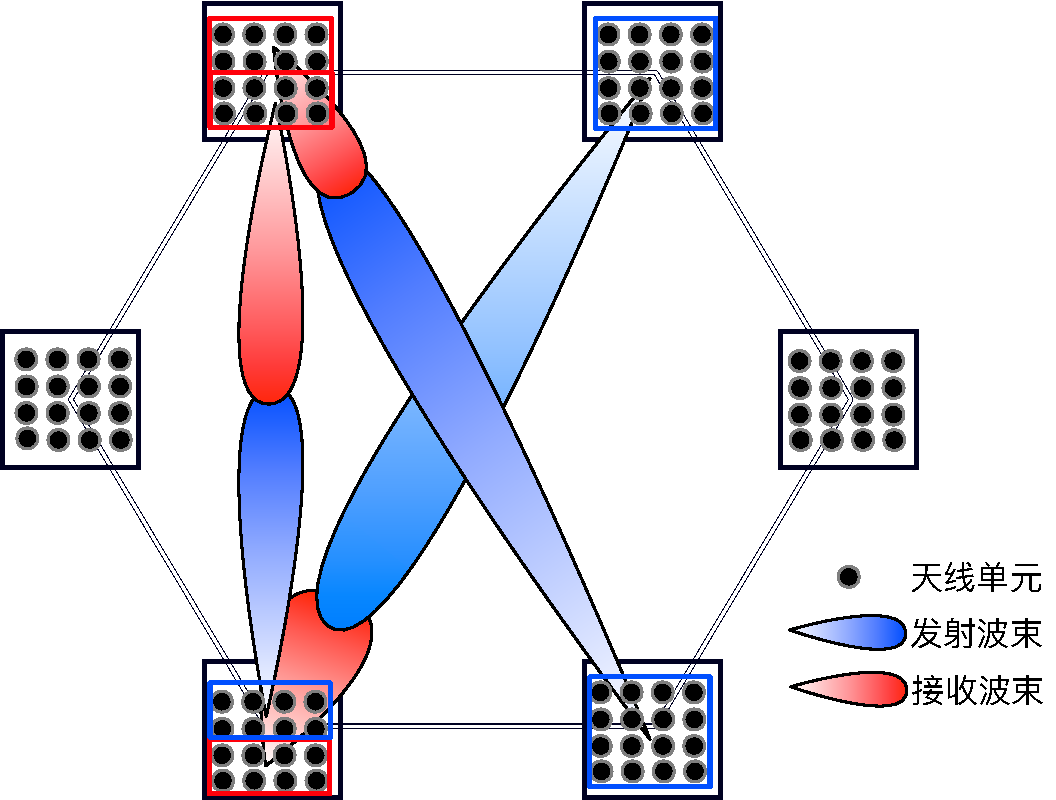
\includegraphics[width=0.7\textwidth]{Pictures/TorBF.pdf}
	\caption{基于毫米波点对点通信的无线数据中心网络}
	\label{fig:TorBF}
\end{figure}

设天线阵列上每个用于通信的均匀线性子阵列的天线单元(Antenna Unit)数量为$n$,则可以得到该阵列的发射/接收增益为

\begin{equation}
G = G_0 + 10log_{10}(n),
\end{equation}
其中$G_0$为每个天线单元的单天线增益\cite{vardhan201460}。

以上关系可以看出当增加通信所用均匀线性阵列中天线单元数量时,得到的增益也会相应增加(增速变缓)。对于一对收发天线而言,接收信号质量与发送与接收两端的天线阵列均呈正相关。在波束对准的情况下,使用的天线数量越多则收到的信号质量越好。由于每个机架顶端的天线单元数量有限,因此在数据中心网络中通信流量不平衡时,需要通过动态调整每个机架顶端天线阵列与另外机架通信所用的天线数量来得到更好的系统性能。为了使整个系统中的不平衡流量集合传输时间最小,可以将优化目标设置为最小化最大的不平衡流量在网络中的传输时间。
设两个机架顶$i$和$j$之间的不平衡流量为$L_{k}$,其中
\begin{equation}
k := \big\{\{i,j\},i,j\in V\big\}.
\end{equation}

则此流量需要的传输时间为
\begin{equation}
T_{k} = \frac{L_{k}}{Th_{k}},
\end{equation}
其中$Th_{k}$为架顶天线$i$发射到架顶天线$j$的吞吐量(信道容量),设每个机架顶端可用于通信的天线数量相同,均为$M$,总机架数量为$N$,则可以建立如下优化问题:

\begin{equation}\label{eq:4.1}
\begin{split}
&\min \max\, T_{k} \\
&s.t.\quad  \left\{\begin{array}{l}
\sum\limits_{k=1}^{K} x_{ik}\leq M,\quad \forall i,\\
x_{ik}\in[1,M], \quad  \forall i,k\end{array}\right.
\end{split}
\end{equation}

其优化目标$\min \max\ T_{k}$为最小化所有任务中消耗的最长时间。优化变量为每个任务$k$对应的架顶天线对$i$和$j$的传输数据所用的天线数量$x_{ik}$和$x_{jk}$,均为整数变量。第一个限制条件代表任意一个架顶天线所用于任务的天线数量和不能超过其上所拥有的总可用天线数量$M$。第二个限制条件代表每个架顶天线可以使用$1$到$M$个天线来传输任务$k$。

任务$k$的实际吞吐量可以表示为
\begin{equation}
Th_{k}=B\times log_2(1+SNR_{ij}),
\end{equation}
$B$为通信所用理论带宽,$SNR_{ij}$为发射接收双方之间的信噪比。
\begin{equation}
SNR_{ij}=\frac{P_r(ij)}{N_0}.
\end{equation}
其中$P_r(ij)$为接收信号强度,单位为$W$。$N_0$为高斯白噪声,服从$N(\mu,\sigma^2)$分布,其中$\mu = 0$,$\sigma^2=1$。
继续由Friis传播模型与Vandhan的工作\cite{vardhan2014polycell}可得
\begin{equation}
	P_{r}(ij)(dBm)=P_t+G_t+G_r+PL_{ij}.
\end{equation}
其中
\begin{equation}
	G_t = G_0+10log_{10}(x_{ik}),
\end{equation}
\begin{equation}
	G_r = G_0+10log_{10}(x_{jk}).
\end{equation}
$P_t$是发射功率,$G_t$和$G_r$分别是所用天线阵列的发射和接收增益,$G_0$是每个全向天线单元的增益,$PL_{ij} = 20log_{10}(\frac{\lambda}{4\pi d})$为路径损耗。其中$\lambda$为波长,$d$为发射与接收天线间的距离。

\section{天线资源分配算法}

很明显,原问题的优化变量是每个天线阵列对于传输任务$k$所使用的天线数量,因此这是一个整数规划问题。我们可以将原问题的整数优化变量用一个二元变量代替,令$x_{ikn(i)}$为二元决策变量,$x_{ikn(i)}=1$时机架天线$i$使用$n(i)$个天线于任务$k$,否则的话$x_{ikn(i)}=0$。则与原问题类似的最小总完成时间问题可以重新建模为一个二次多维多选择背包(Quadratic Multidimensional Multiple Choice Knapsack Problem)问题。

\begin{equation}
	\begin{split}
		&\max\, z = \sum_{i=1}^{M}\sum_{j=1}^{M}\sum_{k=1}^{K}\sum_{n=1}^{N}p_{kn(i)n(j)}x_{ikn(i)}x_{jkn(j)} \\
		&s.t.\quad  \left\{\begin{array}{l}
		\sum\limits_{k=1}^{K}\sum\limits_{n=1}^{N} A_{n}x_{ikn(i)}\leq M, \quad  i = 1,\dots,N\\
		\sum\limits_{n=1}^{N} x_{ikn(i)}\leq 1,\quad i = 1,\dots,I,k = 1,\dots,K\\
		x_{ikn}\in\{0,1\}, \quad  i=1,\dots,M, k=1,\dots,K, n = 1,\dots,N \end{array}\right.
		\end{split}
\end{equation}

其中$p_{kn(i)n(j)}$为对于任务$k$同时选择$A_n x_{ikn(i)}$的机架天线$i$,和$A_n x_{jkn(j)}$的机架天线$j$时生成的联合(二次)收益,$A_n$代表取$n$时的天线实际数量。
参照上一节可以定义为
\begin{equation}
	p_{kn(i)(j)} = \frac{1}{L_{k}} B\times log_2\left[1+\frac{P_r(ij)}{N_0}\right]
\end{equation}

与上一章不同的是,此问题中的收益由发射和接收两者共同决定,相较于多选择多背包问题而言更加复杂。本问题可以从一个标准的二次多背包问题归约,一个标准的二次多背包问题可以表述为
\begin{equation}
	\begin{split}
		&\max\, z = \sum_{i=1}^{M}\sum_{j=1}^{M}\sum_{k=1}^{K}p_{ij}x_{ik}x_{jk} \\
		&s.t.\quad  \left\{\begin{array}{l}
		\sum\limits_{i=1}^{M} A_{i}x_{ik}\leq N_k, \quad  k = 1,\dots,K\\
		\sum\limits_{k=1}^{K} x_{ik}\leq 1,\quad i = 1,\dots,I\\
		x_{ik}\in\{0,1\}, \quad  i=1,\dots,M, k=1,\dots,K,\end{array}\right.
		\end{split}
\end{equation}
当$x_{ikn} = x_{ik}, \quad n = 1,\dots,N$,且$p_{ijkn} = p_{ij},\quad n = 1,\dots,N, \quad k =1,\dots,K$时,多维多选择项消失,原问题可以转化为一个二次多背包问题,即二次多背包问题是本问题的一个特例。由于二次多背包问题是一个NP-hard问题,则该原问题也是一个NP-hard问题。
类似的对于原问题我们只需要在多项式时间内找到一个近似解。

首先将$Th_{ij}$展开,得到

\begin{equation}
	Th_{ij} = B \times log_2\left(1+C_k\times x_{ik}x_{jk}\right),
\end{equation}
其中
\begin{equation}
	C_k = \frac{10^{1/10\times (P_t+2G_0+PL_{ij})}}{N_0}.
\end{equation}.

则优化目标可以写为
\begin{equation}
	\min \max \quad \frac{1}{log_2[(1+C_k\times x_{ik}x_{jk})^{1/L_k}]}.
\end{equation}

由于$log_2( \cdot )$是单调增的上凸函数,因此可以求解下式得到原问题的解
\begin{equation}\label{eq:newmin}
	\arg  \min  \max \quad (1+C_k\times x_{ik}x_{jk})^{-1/L_k}.
\end{equation}


此时我们在原问题(\ref{eq:newmin})中引入一个变量$\lambda$,令
\begin{equation}
	(1+C_k\times x_{ik}x_{jk})^{-1/L_k}\leq \lambda,\quad \forall k.
\end{equation}

由于括号内$C_k\times x_{ik}x_{jk}>>1$,因此可以将括号内的$1$忽略掉,得到
\begin{equation}
C^{-1/L_k}\times x_{ik}^{-1/L_k} \times x_{jk}^{-1/L_k} \times \lambda^{-1} \leq 1.
\end{equation}

此时可以将优化问题重新写为

\begin{equation}\label{eq:newone}
\begin{split}
&\min \quad\lambda \\
&s.t.\quad  \left\{\begin{array}{lr}
C^{-1/L_k}\times x_{ik}^{-1/L_k} \times x_{jk}^{-1/L_k} \times \lambda^{-1} \leq 1, &\forall k\\
\sum\limits_{k=1}^{K}M^{-1}x_{ik} \leq 1, \quad &\forall i\\
\sum\limits_{k=1}^{K}M^{-1}x_{jk} \leq 1, \quad &\forall j\\
x_{ik}\in[1,M], \quad  &\forall i,k \end{array}\right.
\end{split}
\end{equation}

其中$C^{-1/L_k}>0$。我们将整数优化变量$x_{ik},x_{jk}$松弛成实数域上的连续变量,此时该问题可被看作是一几何规划问题。
由于变量$x_{ik},x_{jk} > 0$,因此可以
继续利用$y_i =  \log x_i$进行变量替换,即$x_i = e^{y_i}$。此时原问题可以转换为一凸优化问题,进而可以通过一些成熟的优化工具箱,如MOSEK\cite{mosek}进行求解,将得到的解通过取整的方式即可得到次优的整数解。

\section{仿真验证}

本章仿真实验均在一台频率为3.2GHz的Intel\textregistered ~ Core\texttrademark ~ i5-4570 CPU的计算机上,利用MATLAB\textregistered 实现。
假设数据中心网络中有共200个机架,在某一时刻有一组容量为$L_{k}$的任务需要在网络中传输,$L_{k}:=load_{ij}$可以表示为一个归一化后的连接权重矩阵,按照一定的不平衡分布随机生成。所用毫米波频率为$60$GHz,天线阵列上的天线单元间距离为半波长,即$5$毫米。
设任意两个架顶天线通信时的发射功率为$P_t = 40dBm$,每个天线单元的基础增益$G_0 = 6dB$。

如图(\ref{fig:dn})所示,每个架顶天线上的总可用天线单元数量与所有任务的最小最大完成时间的关系。显然随着天线数量的增加,最小最大完成时间逐渐下降。但是由于天线数量的增加所带来的增益增速会逐渐降低,导致完成时延的降低速率也逐渐变缓。

\begin{figure}[htbp]
	\centering
	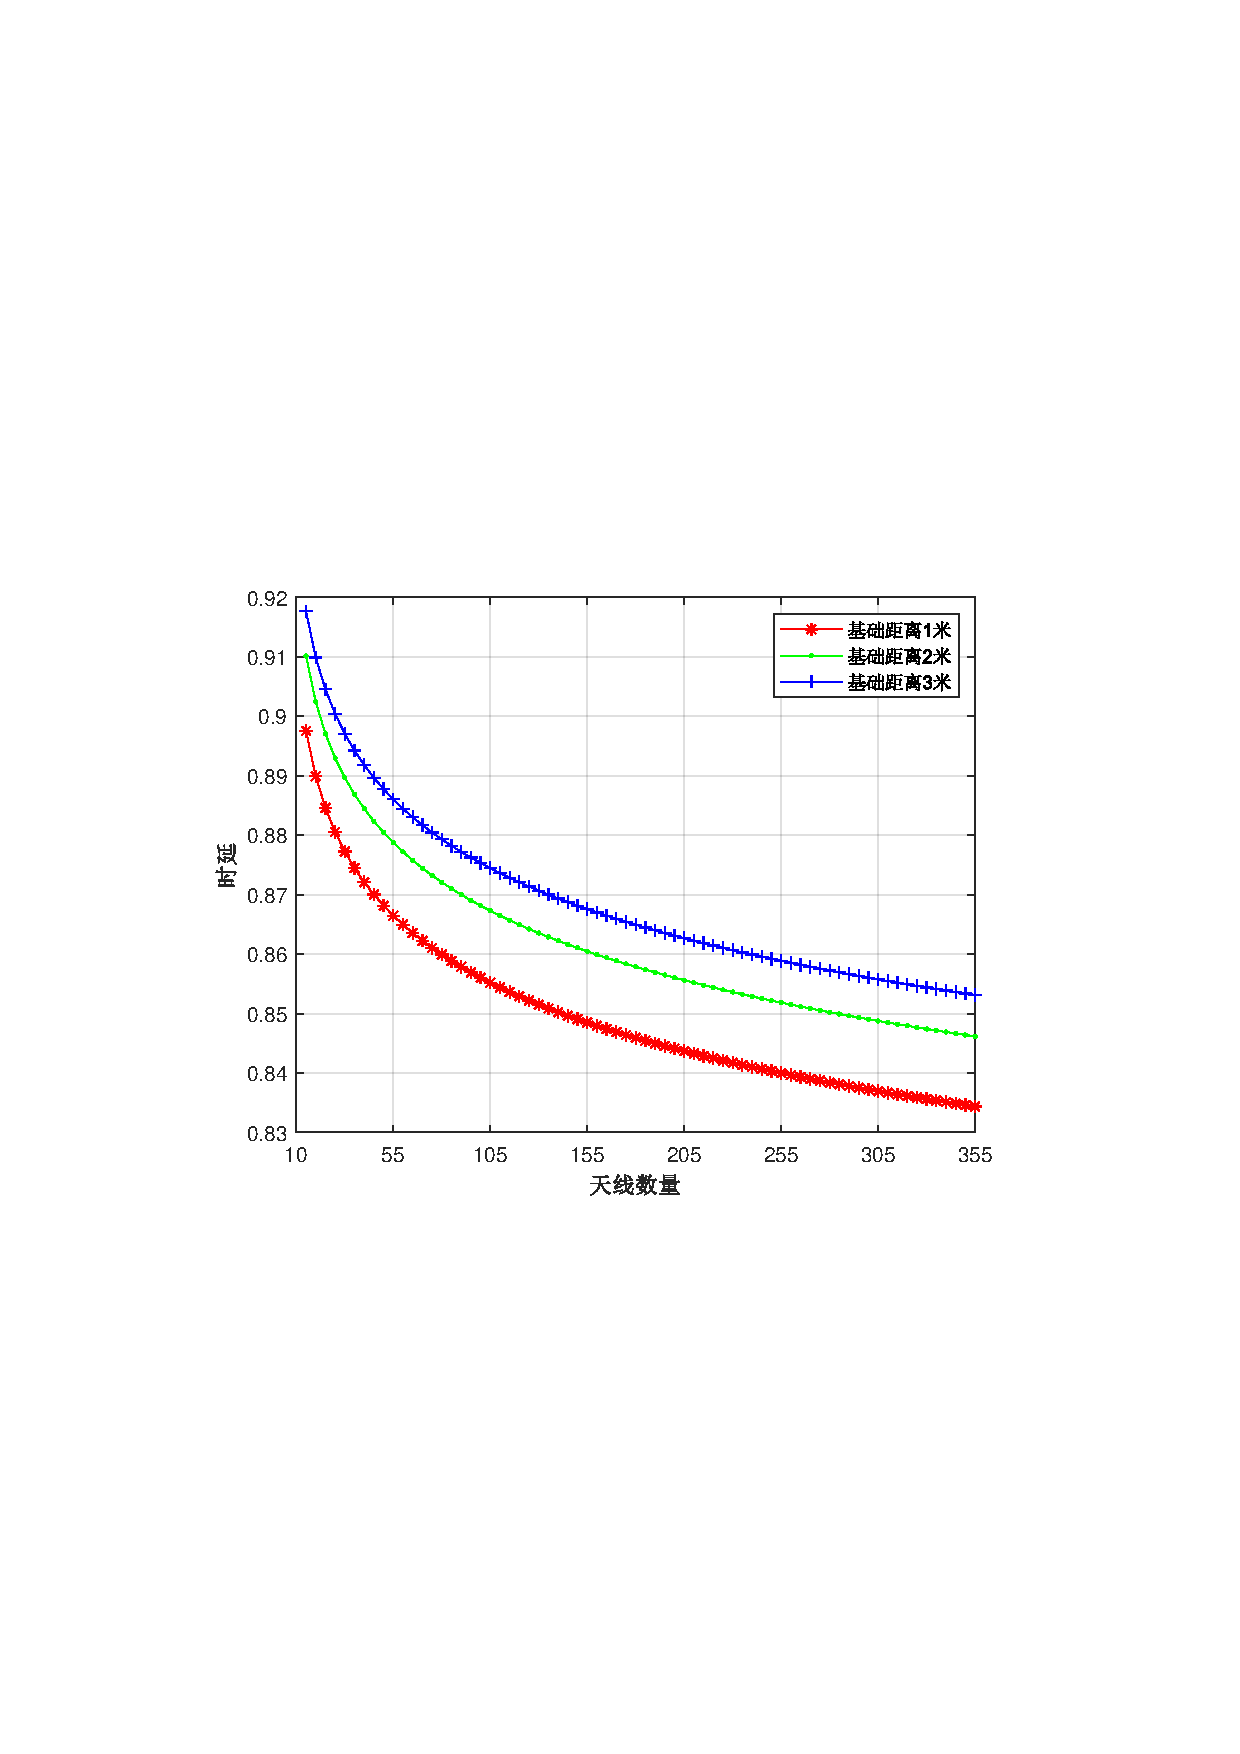
\includegraphics[width=0.7\textwidth]{Pictures/Dnumber.pdf}
	\caption{不同架顶天线可用数量时的性能比较曲线图}
	\label{fig:dn}
\end{figure}

如图(\ref{fig:dd})所示,架顶天线间的基础(最小)距离与所有任务的最小最大完成时间的关系。显然随着基础距离的增加,毫米波信号在空间中的衰减也逐渐增加,最小最大完成时间逐渐升高。随着距离的增加,这种升高的趋势逐渐变慢。

\begin{figure}[htbp]
	\centering
	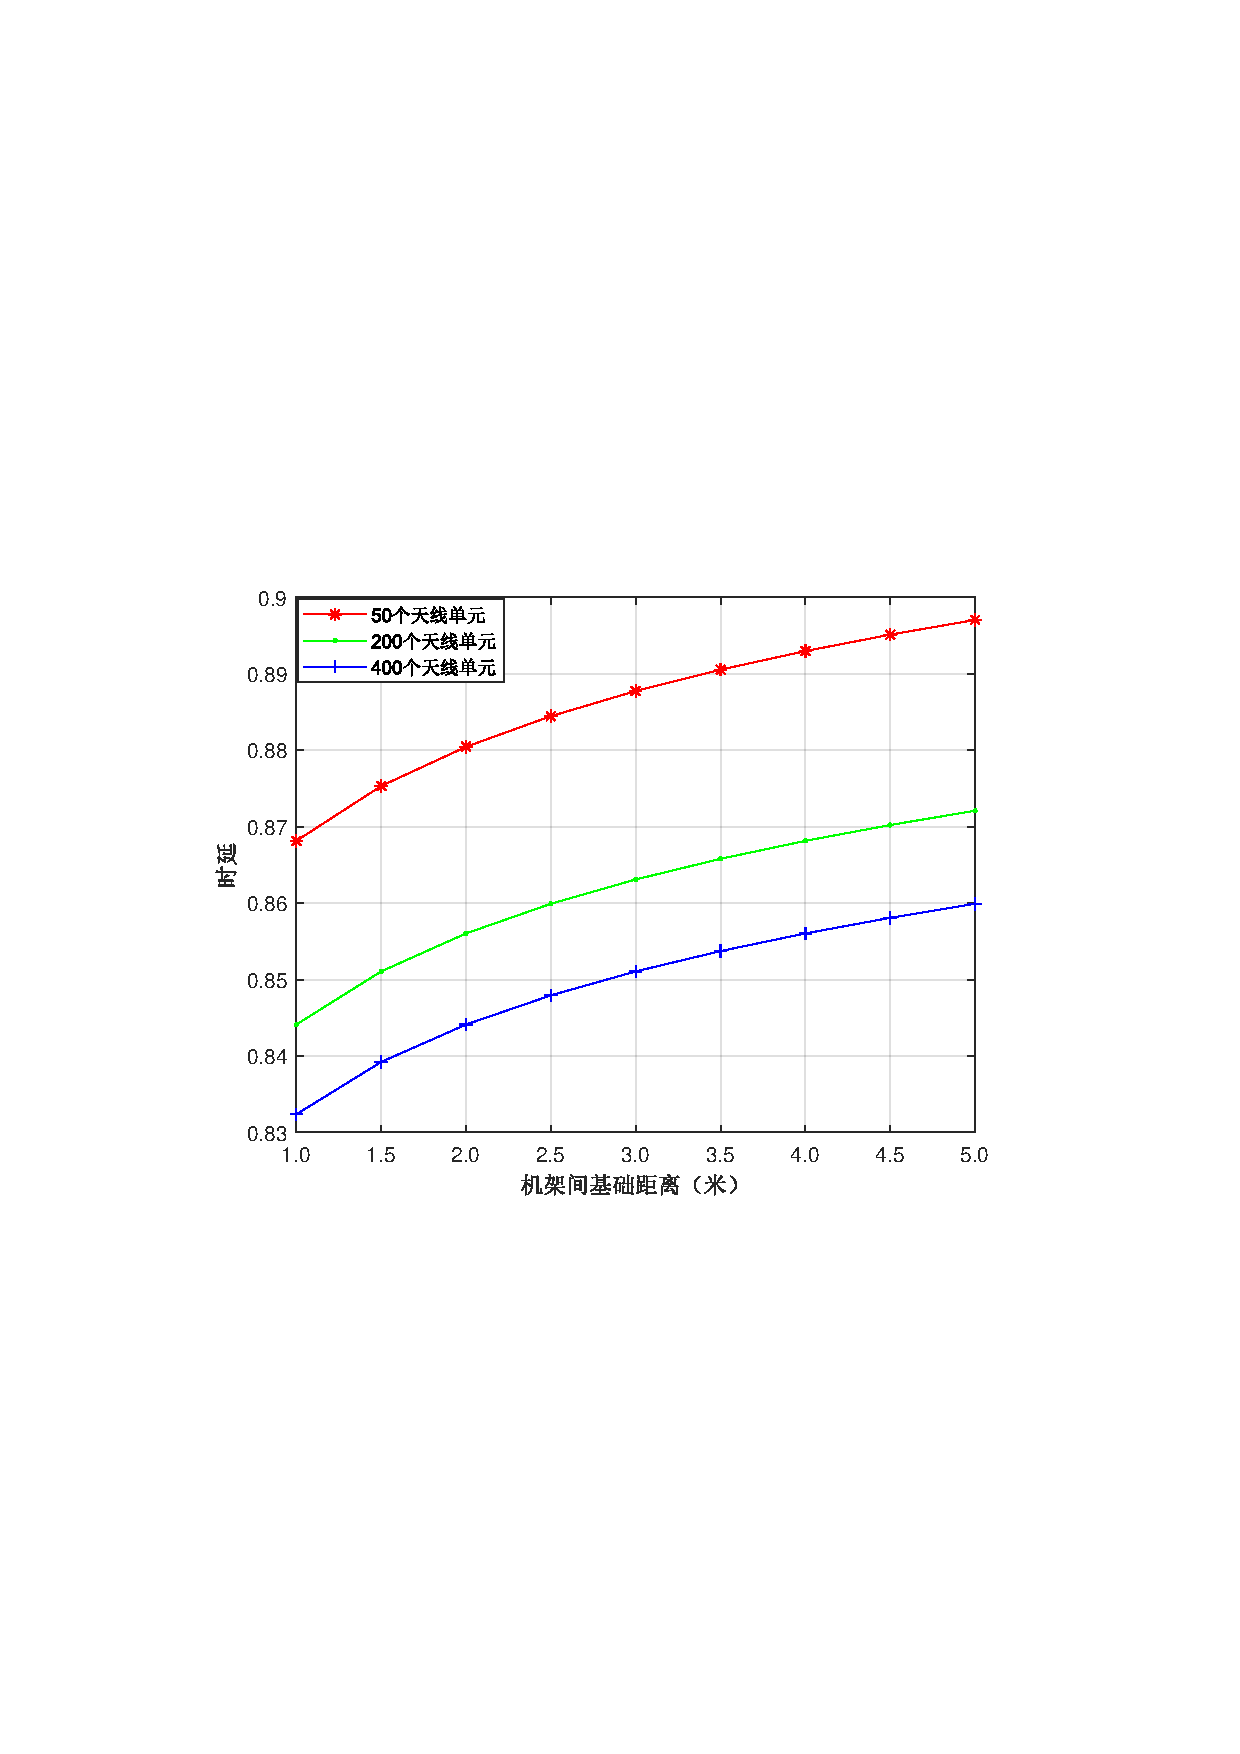
\includegraphics[width=0.7\textwidth]{Pictures/Distance.pdf}
	\caption{不同机架间基础距离时的性能比较曲线图}
	\label{fig:dd}
\end{figure}

在以上单层网络的仿真结果基础上,进行三层网络与单层网络传输效果的比较。设三层网络中每层天线所在的水平面间的距离差为$0.5$米。最大通信范围设为$3$倍的机架间基础距离,此时任意节点通信范围内的邻居个数增加到$14$个。事实上,三层网络中任意一点$i$与其新加入邻居节点$j$间,在对应的单层网络中一定存在一个公共邻居节点$k$。则其对应的连接可以通过单层网络中的公共邻居节点$k$进行转发,即将原有任务$L_{ij}$拆分为$L_{ik}$和$L_{kj}$,其中$L_{ij}=L_{ik}=L_{kj}$。

如图(\ref{fig:3to1})所示为两种网络结构下每个架顶天线上的总可用天线单元数量与所有任务的最小最大完成时间的关系。同样随着天线数量的增加,最小最大完成时间逐渐下降。同时可以看出三层网络的传输性能要好于单层网络。

\begin{figure}[htbp]
	\centering
	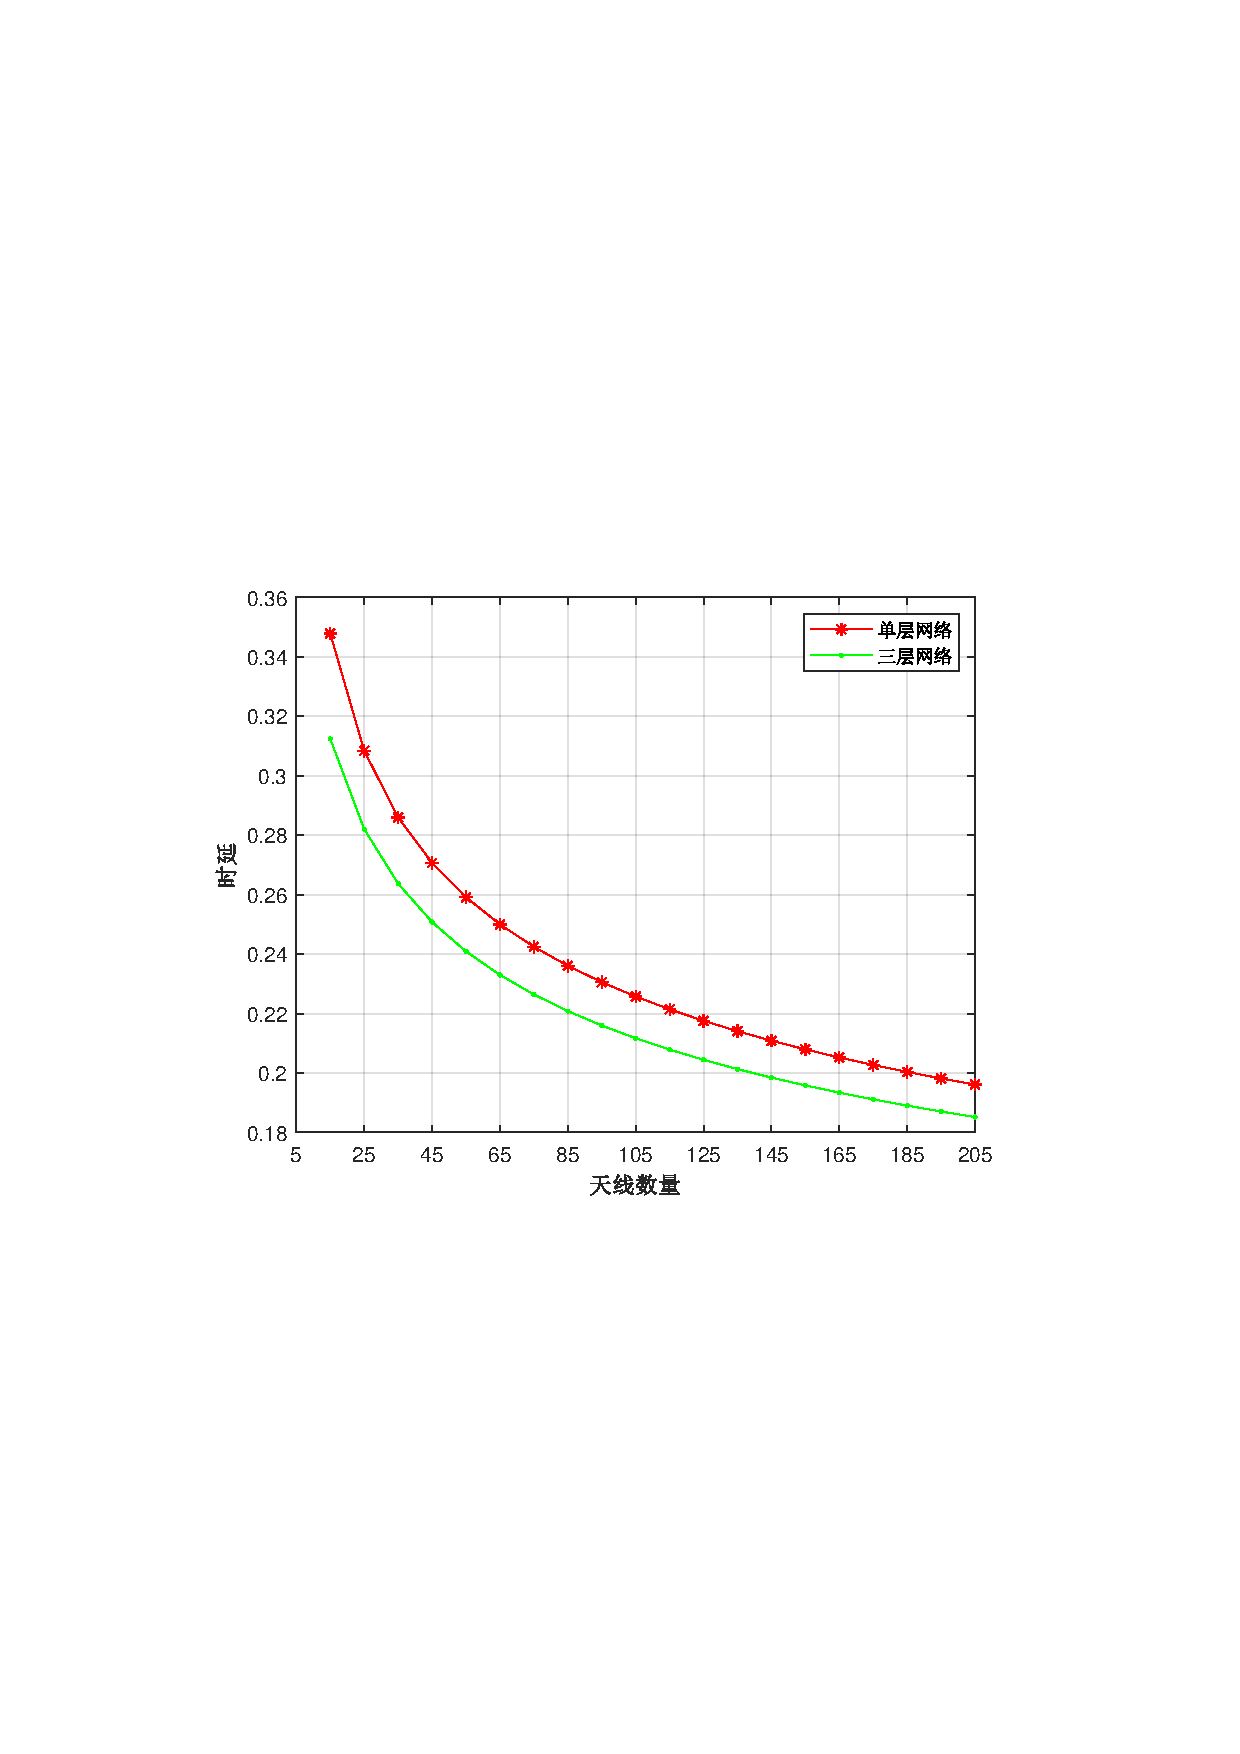
\includegraphics[width=0.7\textwidth]{Pictures/3to1.pdf}
	\caption{三层网络与单层网络在不同天线数量时的性能比较曲线图}
	\label{fig:3to1}
\end{figure}

如图(\ref{fig:3to})所示为两种网络结构下不同机架间基础距离与所有任务的最小最大完成时间的关系。显然随着距离的增加,最小最大完成时间逐渐下降。可以看出由于三层网络结构下每个机架能够直接通信的机架数量增多,使得三层网络的传输性能要好于单层网络。

\begin{figure}[htbp]
	\centering
	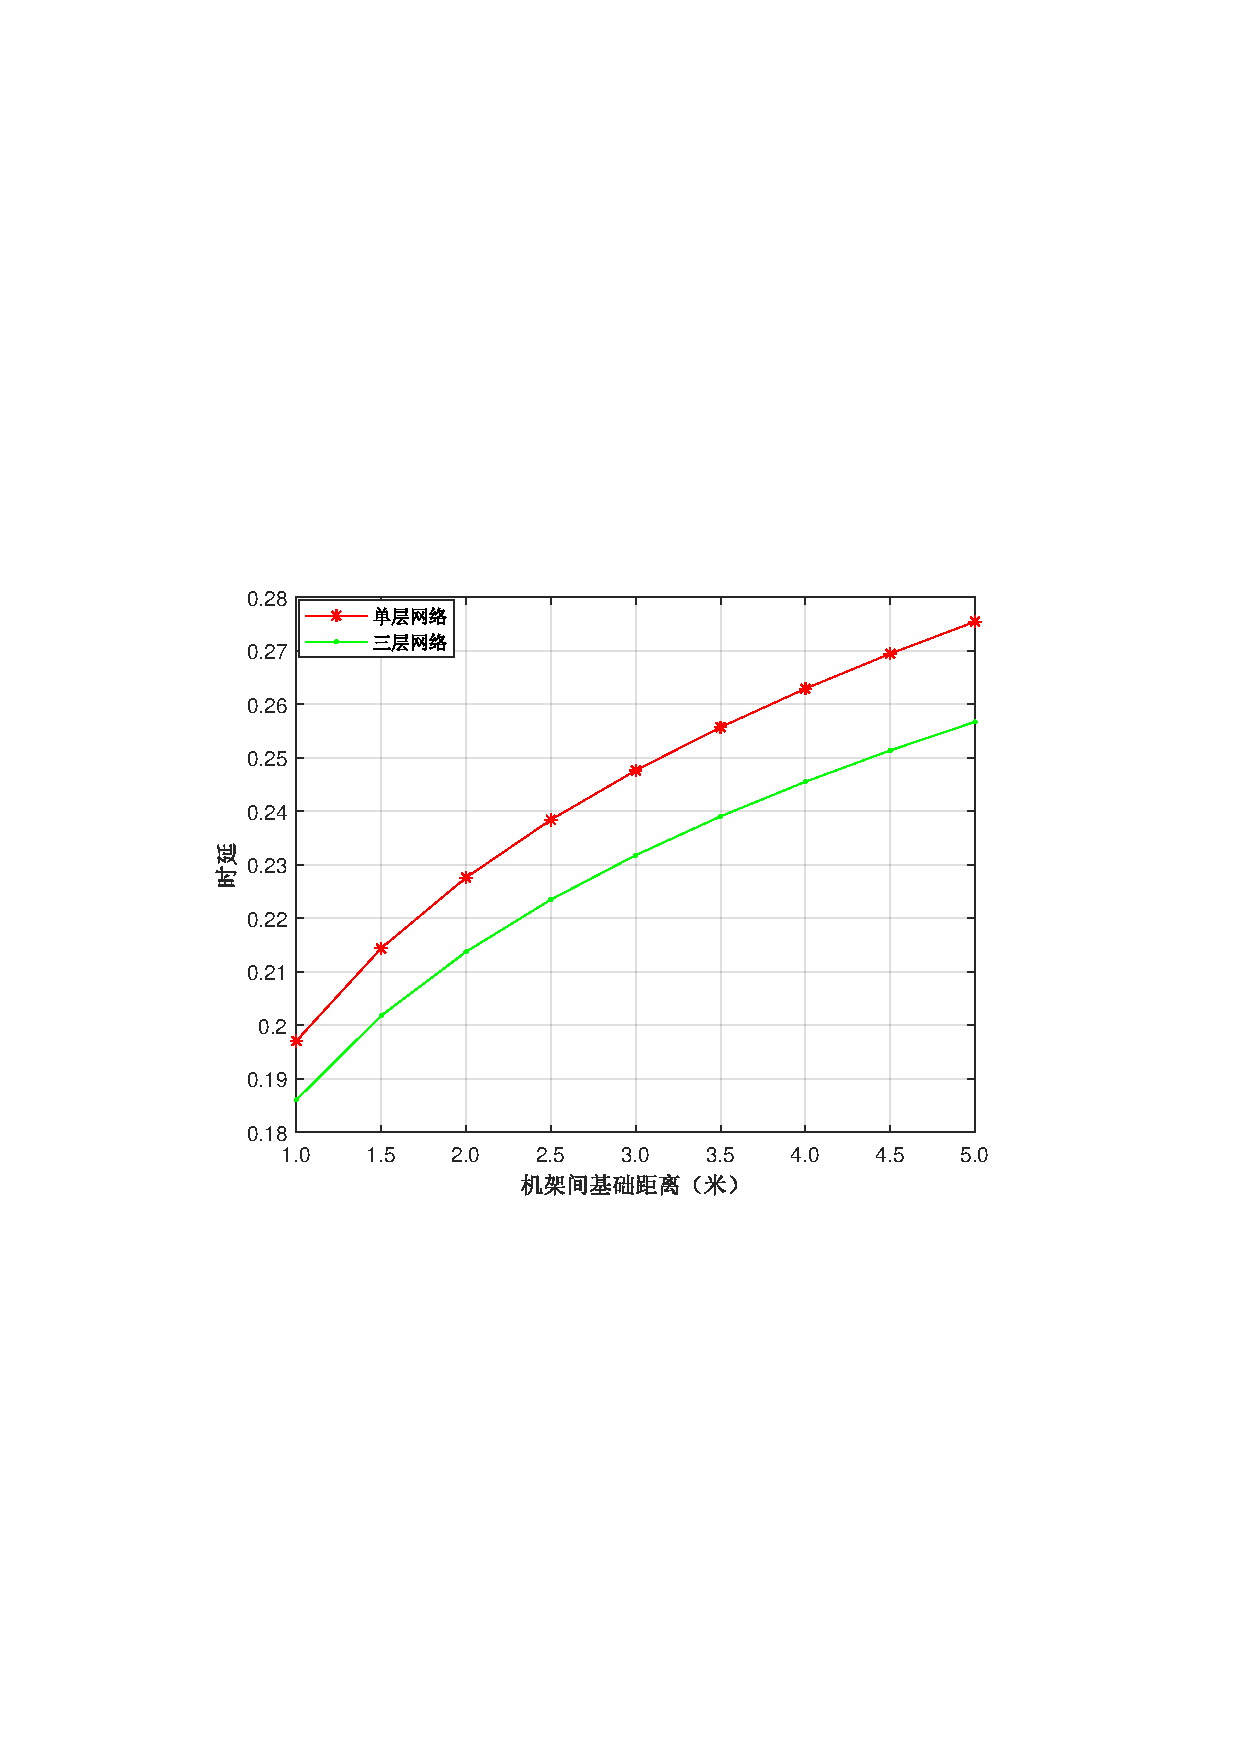
\includegraphics[width=0.7\textwidth]{Pictures/3to.pdf}
	\caption{三层网络与单层网络在不同机架间基础距离时的性能比较曲线图}
	\label{fig:3to}
\end{figure}


如图(\ref{fig:yjd})所示为两种网络结构下不同流量拥挤度与所有任务的最小最大完成时间的关系。横轴显示的是不同比例的流量集中在$25\%$的机架之间,比例越高则有更多的流量集中在这$25\%$的机架中。显然随着流量拥挤度的增加,最小最大完成时间逐渐上升。可以看出由于三层网络结构下每个机架能够直接通信的机架数量增多,使得三层网络的传输性能要好于单层网络。

\begin{figure}[htbp]
	\centering
	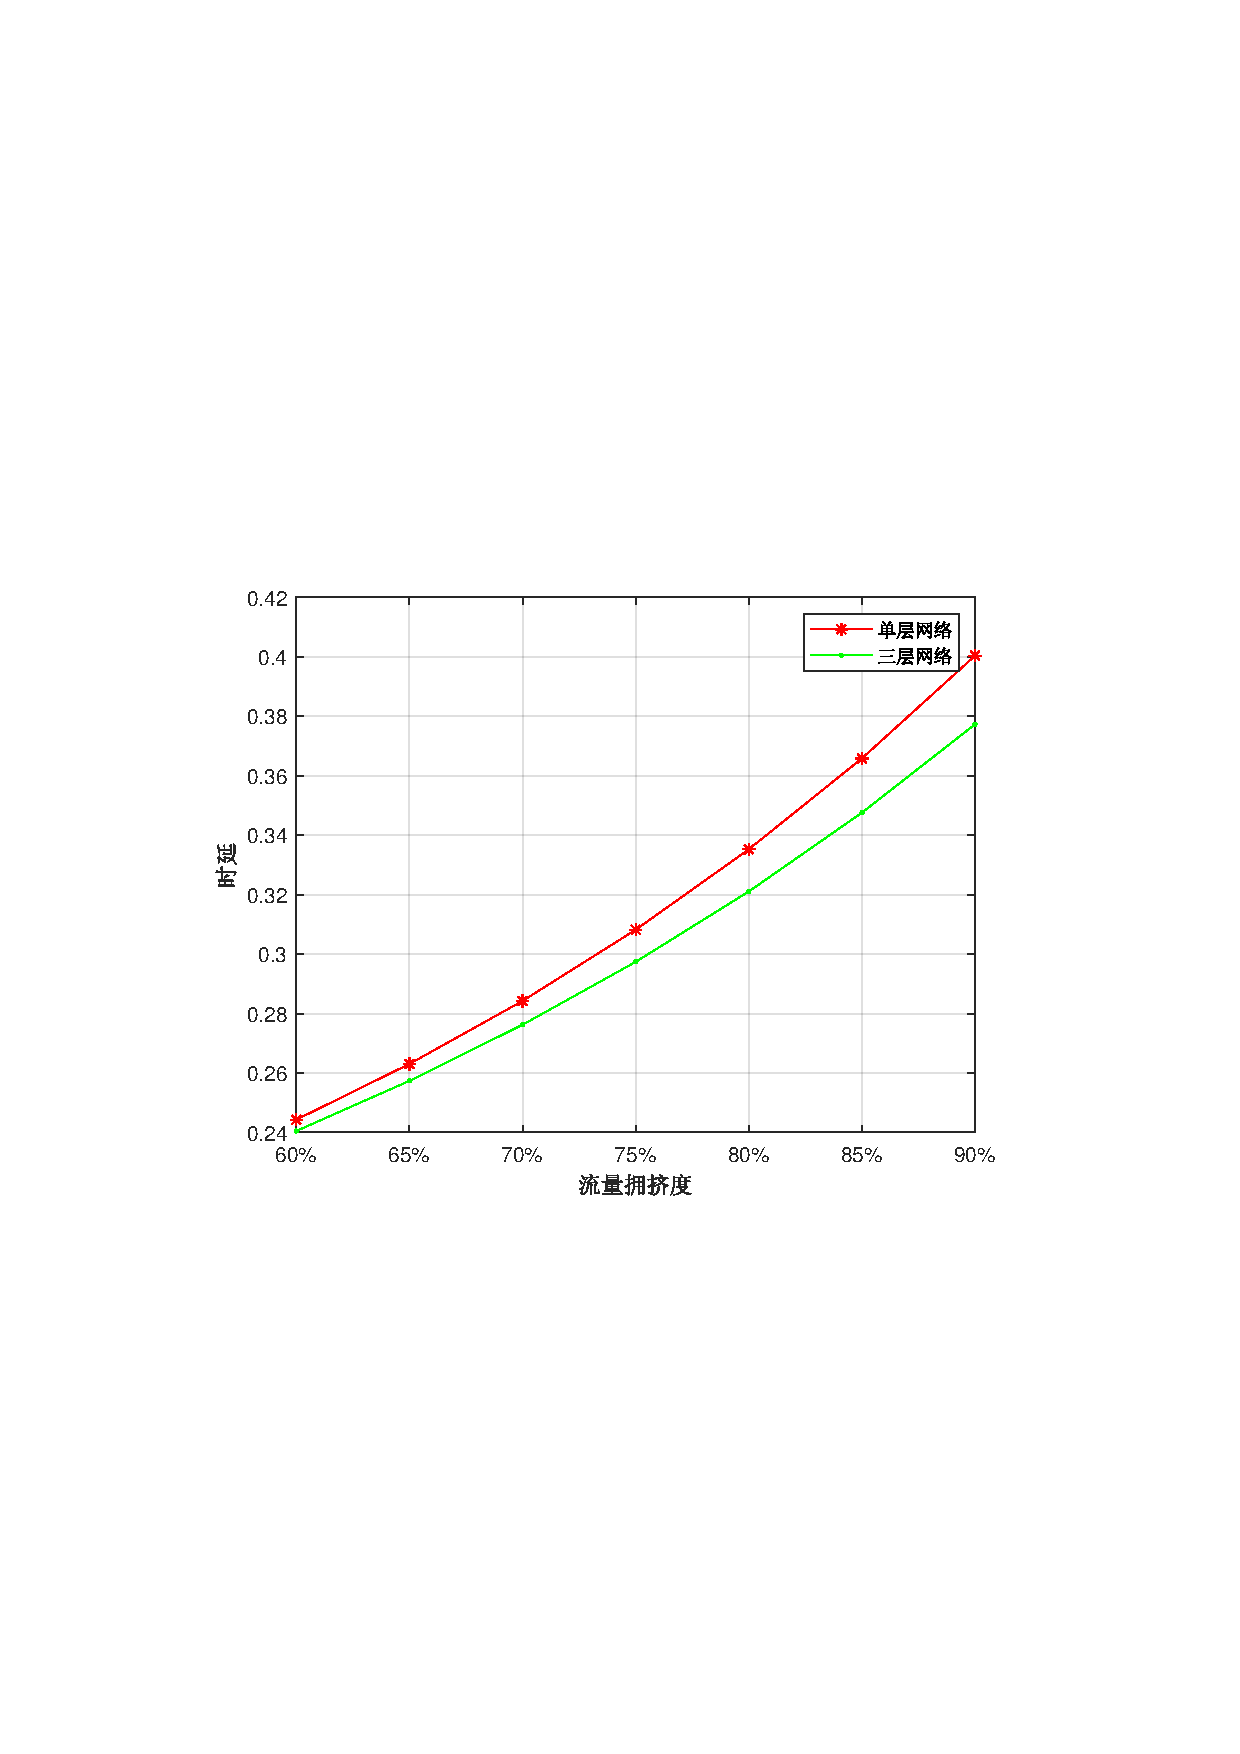
\includegraphics[width=0.7\textwidth]{Pictures/yjd.pdf}
	\caption{三层网络与单层网络在不同流量拥挤度时的性能比较曲线图}
	\label{fig:yjd}
\end{figure}

如图(\ref{fig:yjd2})所示为两种网络结构下不同流量集中度与所有任务的最小最大完成时间的关系。横轴显示的是$80\%$的流量集中在不同比例的机架之间,比例越低则流量的流向越集中。显然随着流量集中度的增加,最小最大完成时间逐渐上升,但三层网络的传输性能要好于单层网络。

\begin{figure}[htbp]
	\centering
	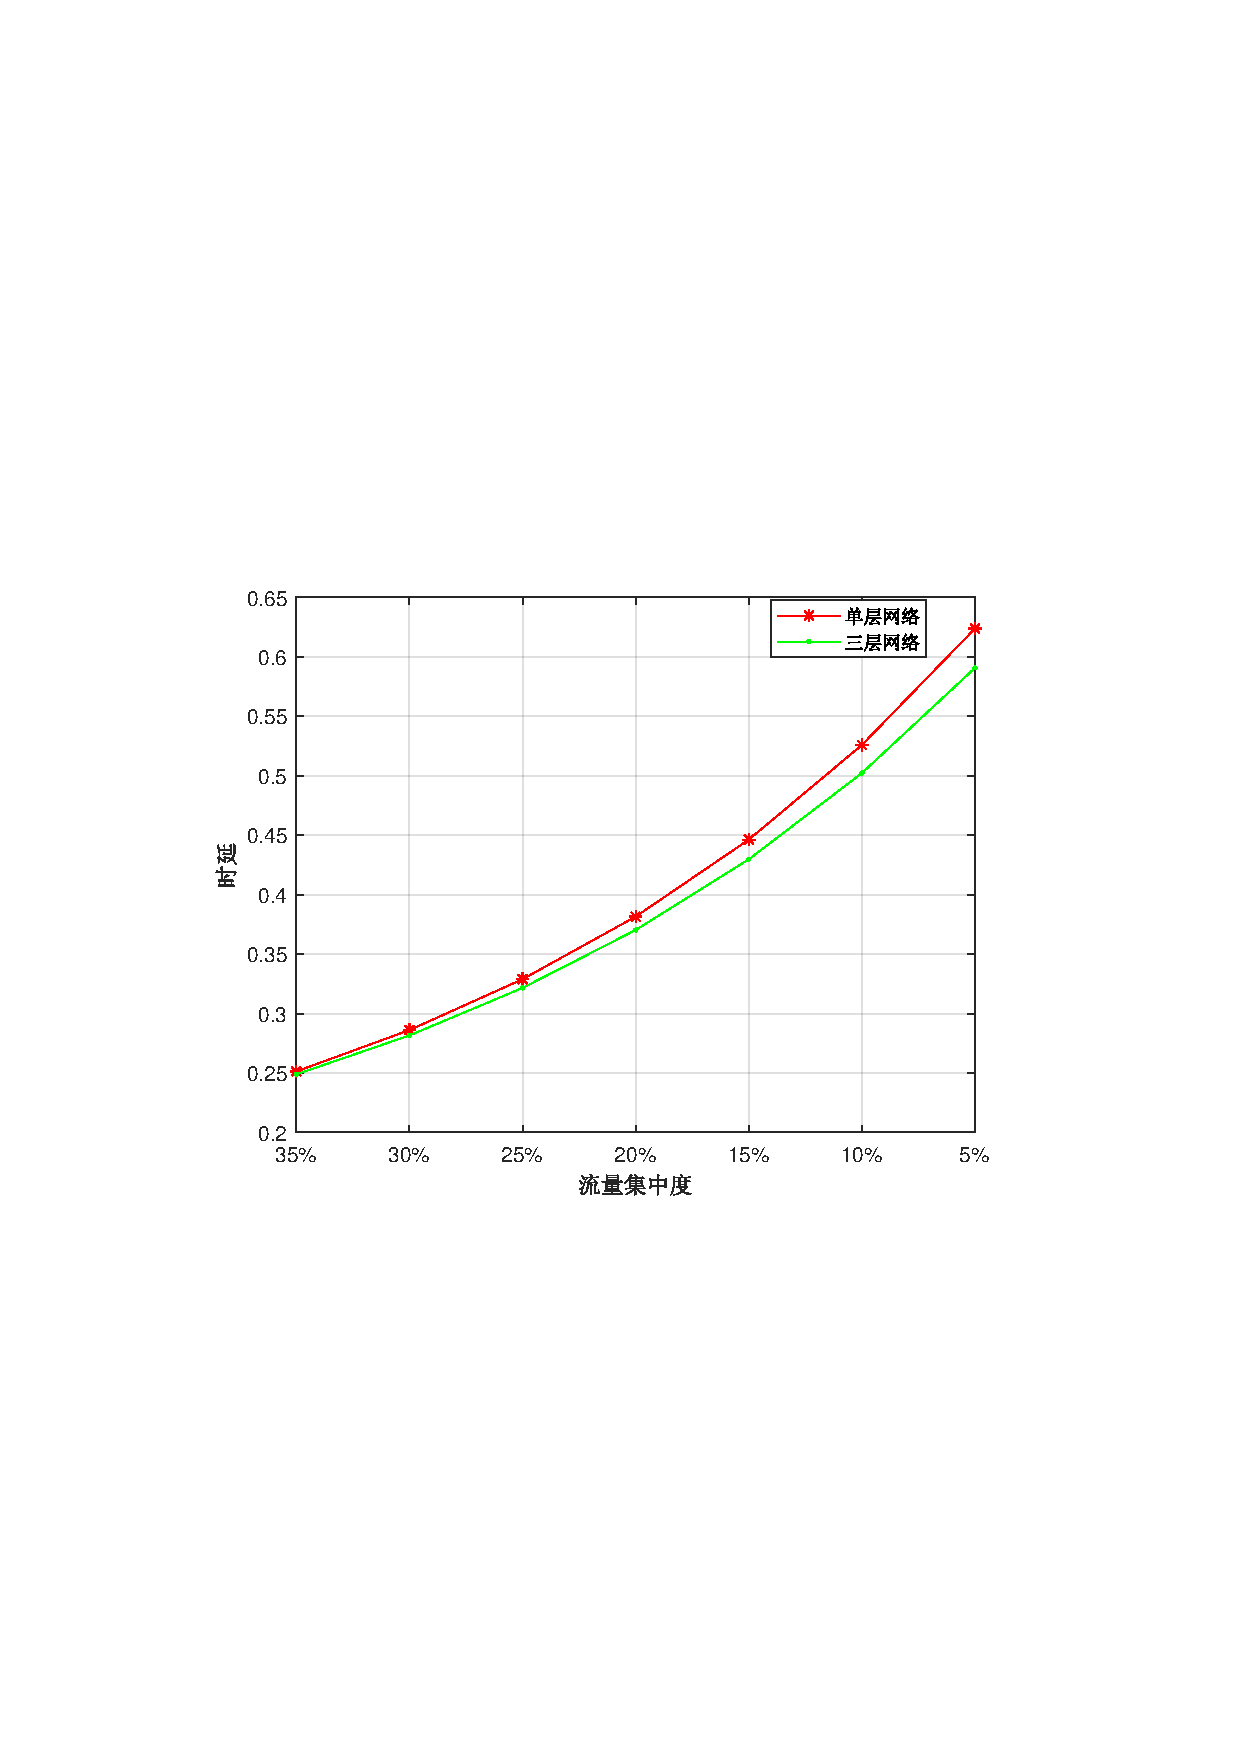
\includegraphics[width=0.7\textwidth]{Pictures/yjd2.pdf}
	\caption{三层网络与单层网络在不同流量集中度时的性能比较曲线图}
	\label{fig:yjd2}
\end{figure}

\section{本章小结}
本章研究了毫米波通信应用在数据中心网络这一典型网状网络场景中的资源优化分配问题。随着近些年数据中心网络中网络流量性质的变化,网络中逐渐出现了严重的流量不平衡现象,降低了数据中心网络的通信性能。为了减少这些不平衡流量带来的通信延时问题,本章将毫米波通信应用在数据中心网络中,以点对点无线通信的方式传输不平衡流量。通过在服务器机架顶上安置毫米波阵列天线,使得一定范围内的服务器架顶间可以直接通过毫米波信号相互通信。根据毫米波阵列天线的特点与视距通信的要求,将机架按照正六边形的形式放置,并在单层和三层两种场景下建立了毫米波无线数据中心网络拓扑结构。在此基础上对每个架顶的天线资源进行优化分配问题建模,通过变量替换等方式将问题转化为几何规划问题并求解,降低了在一定流量负荷情况下的网络最大通信时延。仿真结果验证了提出的毫米波无线数据中心网络结构与优化算法的有效性。

